\chapter{Additional Figures}
\label{ap:addFig}
 
\section{Integrated Autocorrelation plots} 
\subsection{Ozone}
\begin{figure}[ht!]
	\centering
	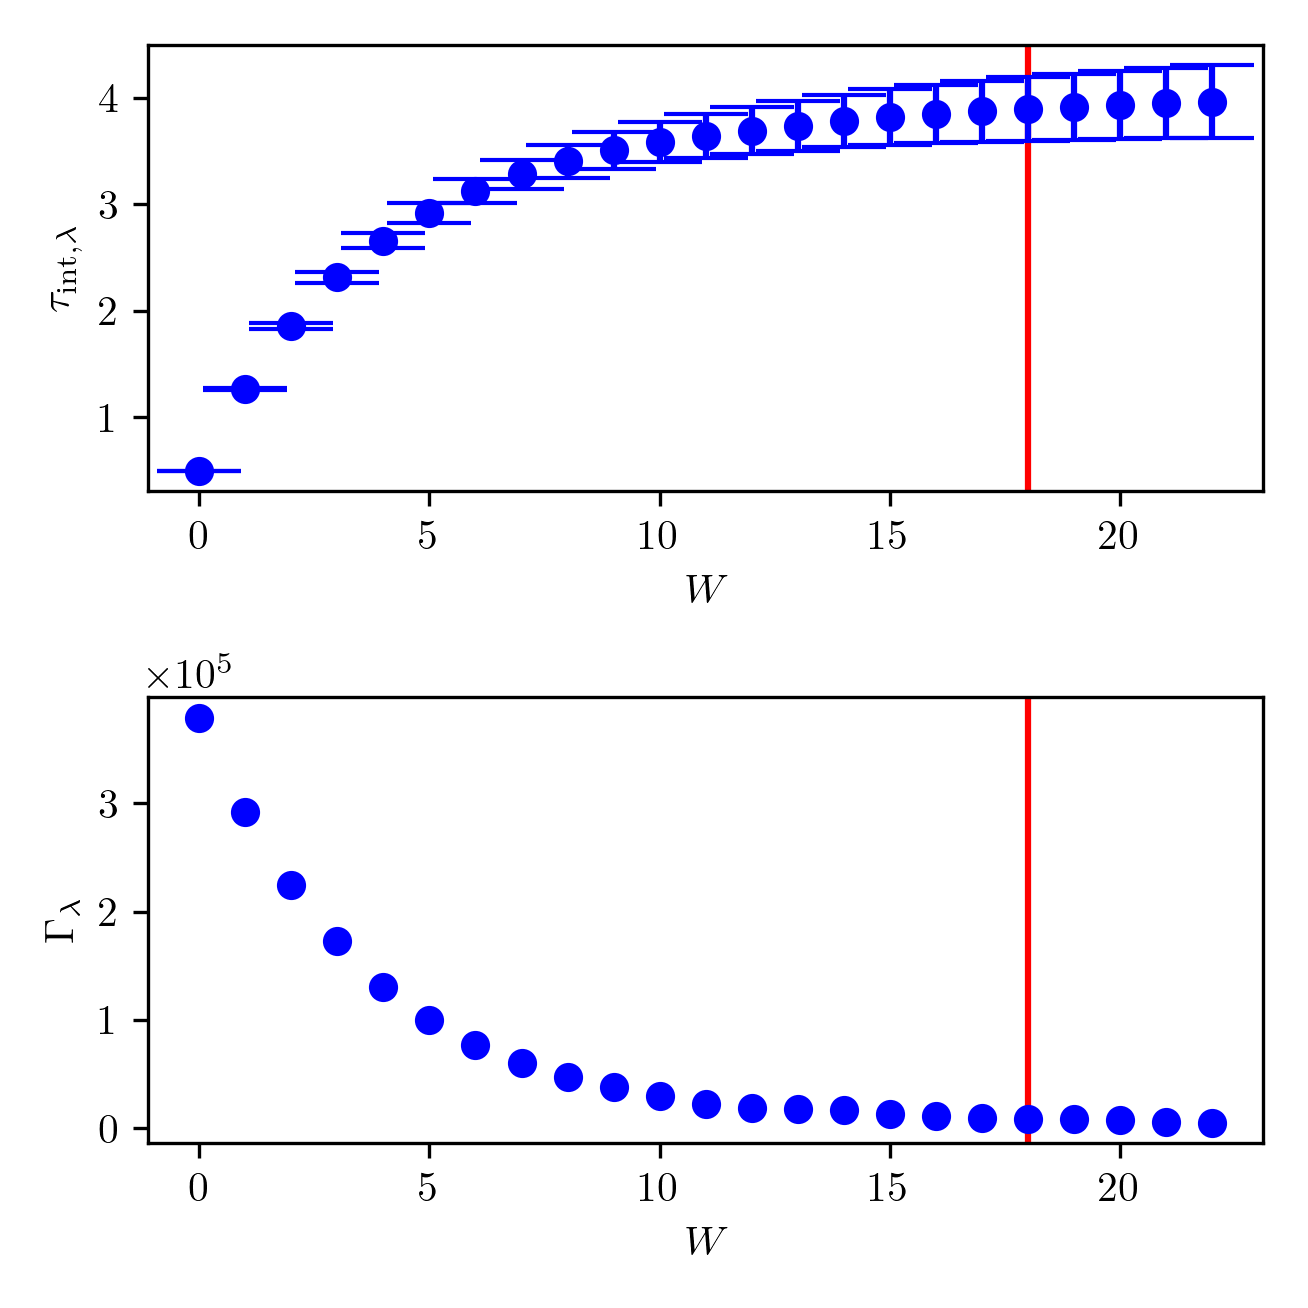
\includegraphics{UwerrTauIntSecO3lam.png}
	\caption[]{}
	\label{fig:}
\end{figure}
\begin{figure}[ht!]
	\centering
	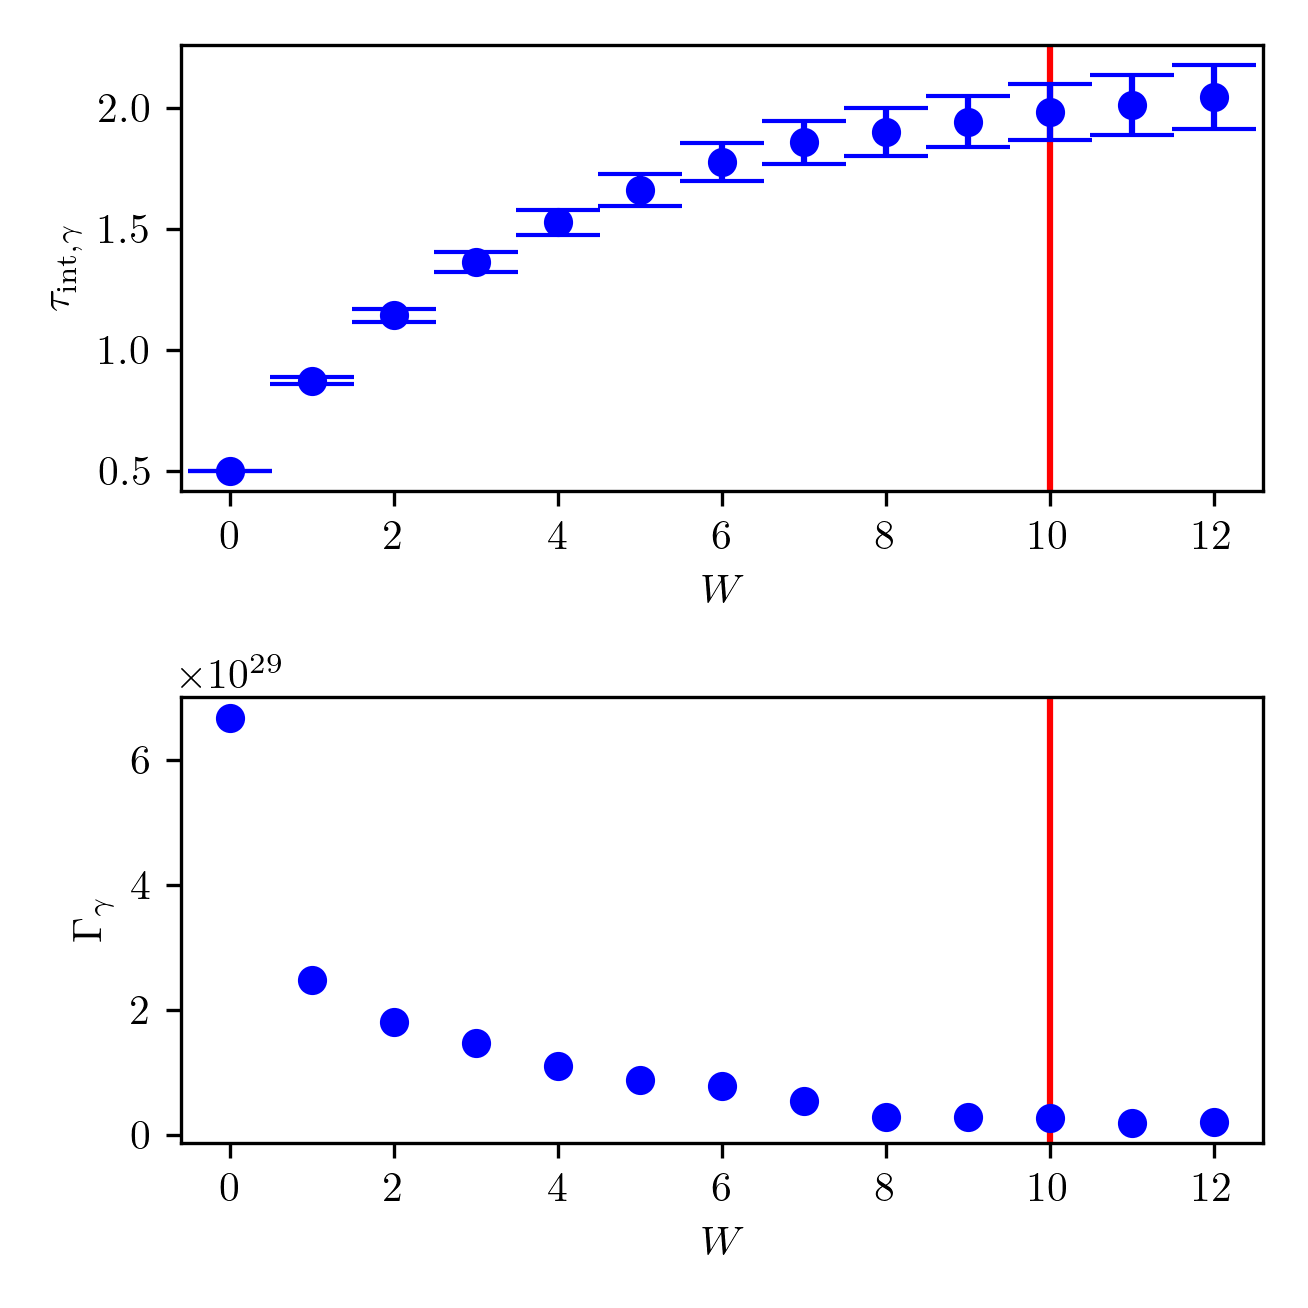
\includegraphics{UwerrTauIntSecO3gam.png}
	\caption[]{}
	\label{fig:}
\end{figure}
\subsection{Pressure and Temperature}
\begin{figure}[ht!]
	\centering
	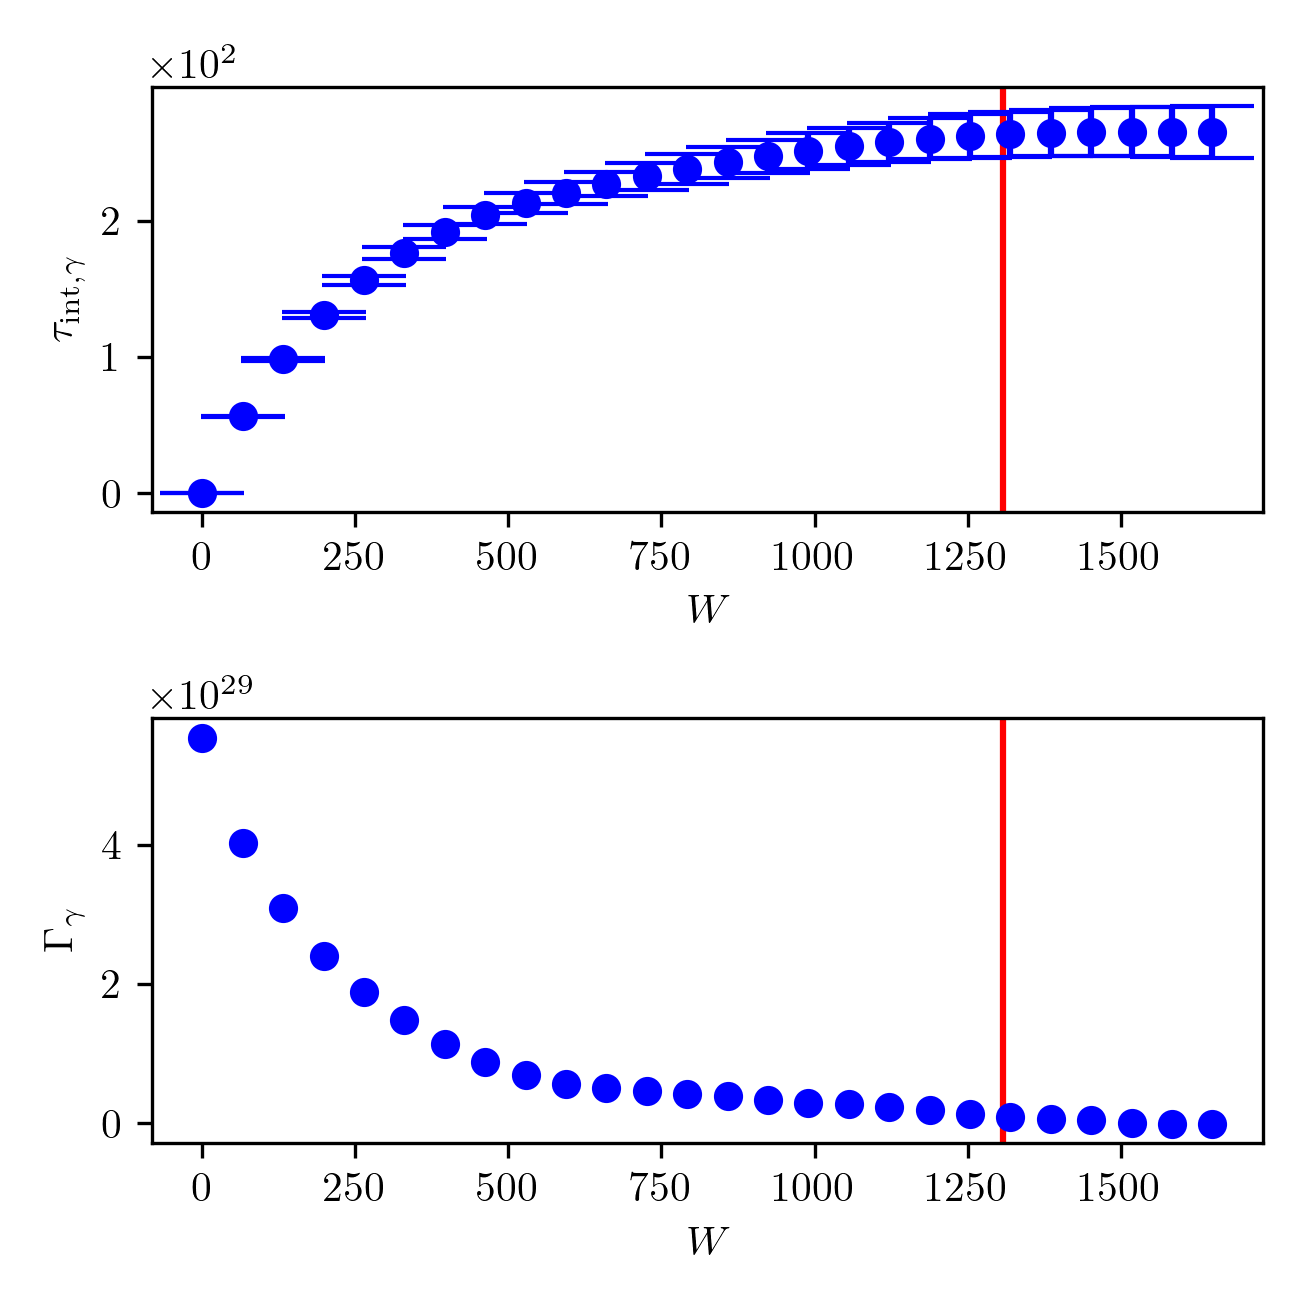
\includegraphics{UwerrTauIntTWalk0.png}
	\caption[]{}
	\label{fig:}
\end{figure}
\begin{figure}[ht!]
	\centering
	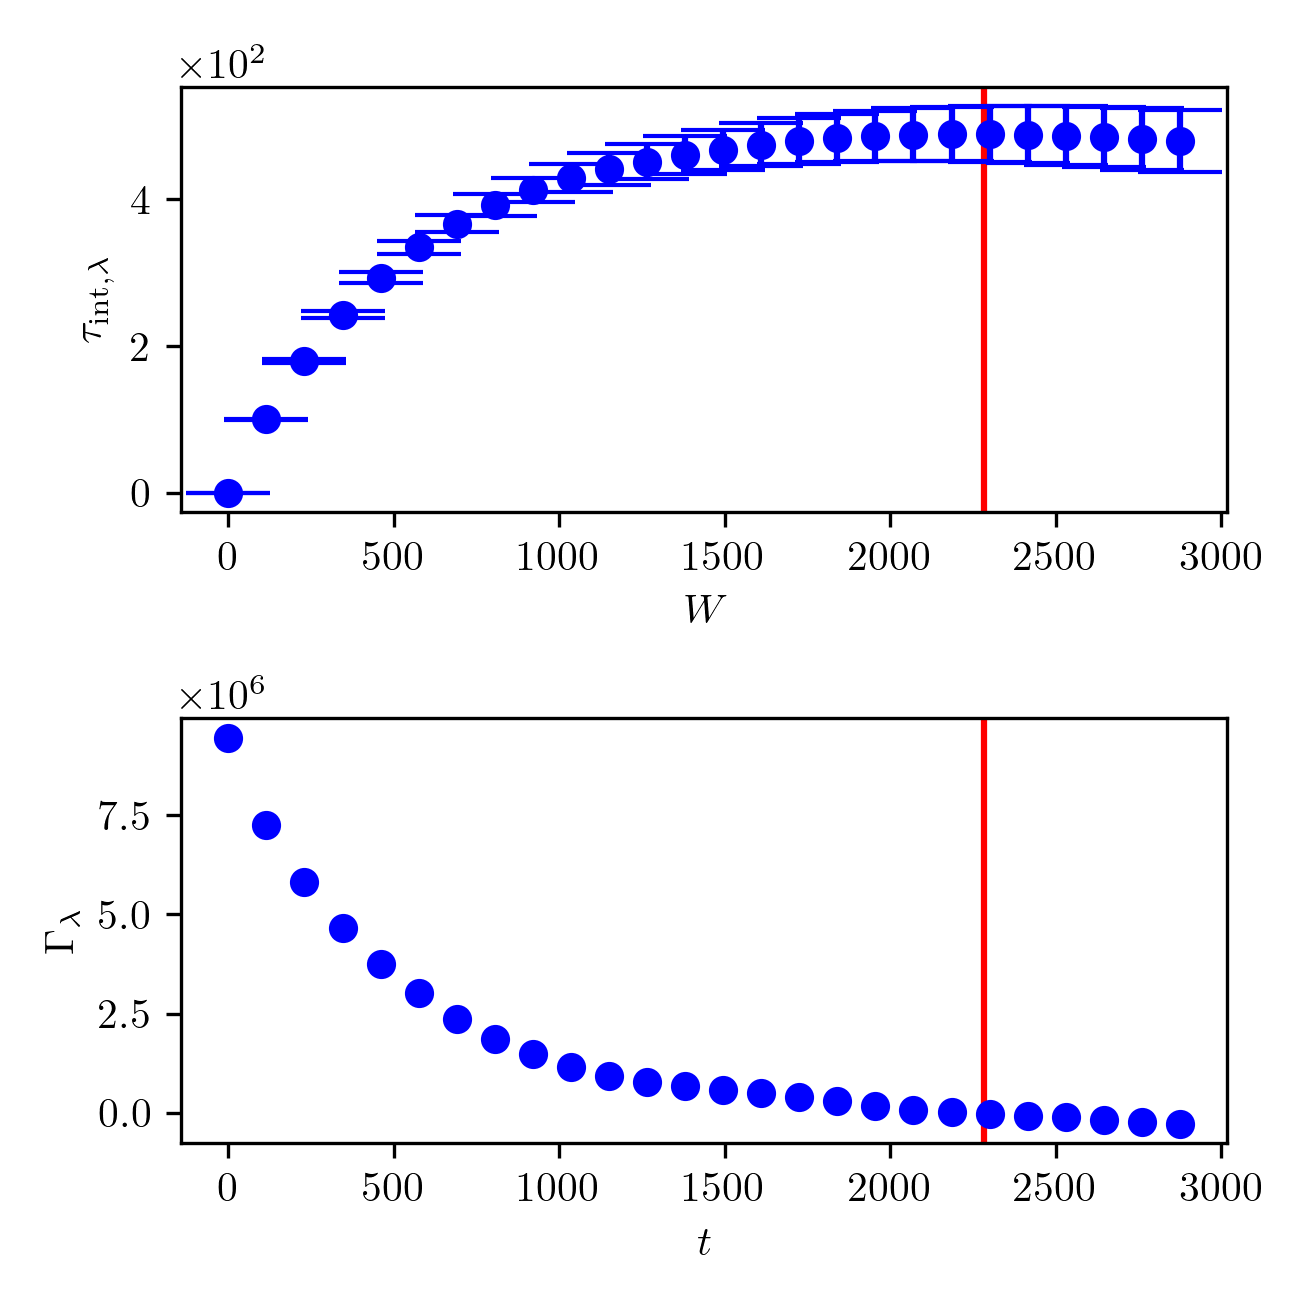
\includegraphics{UwerrTauIntTWalk1.png}
	\caption[]{}
	\label{fig:}
\end{figure}


\begin{figure}[ht!]
	\centering
	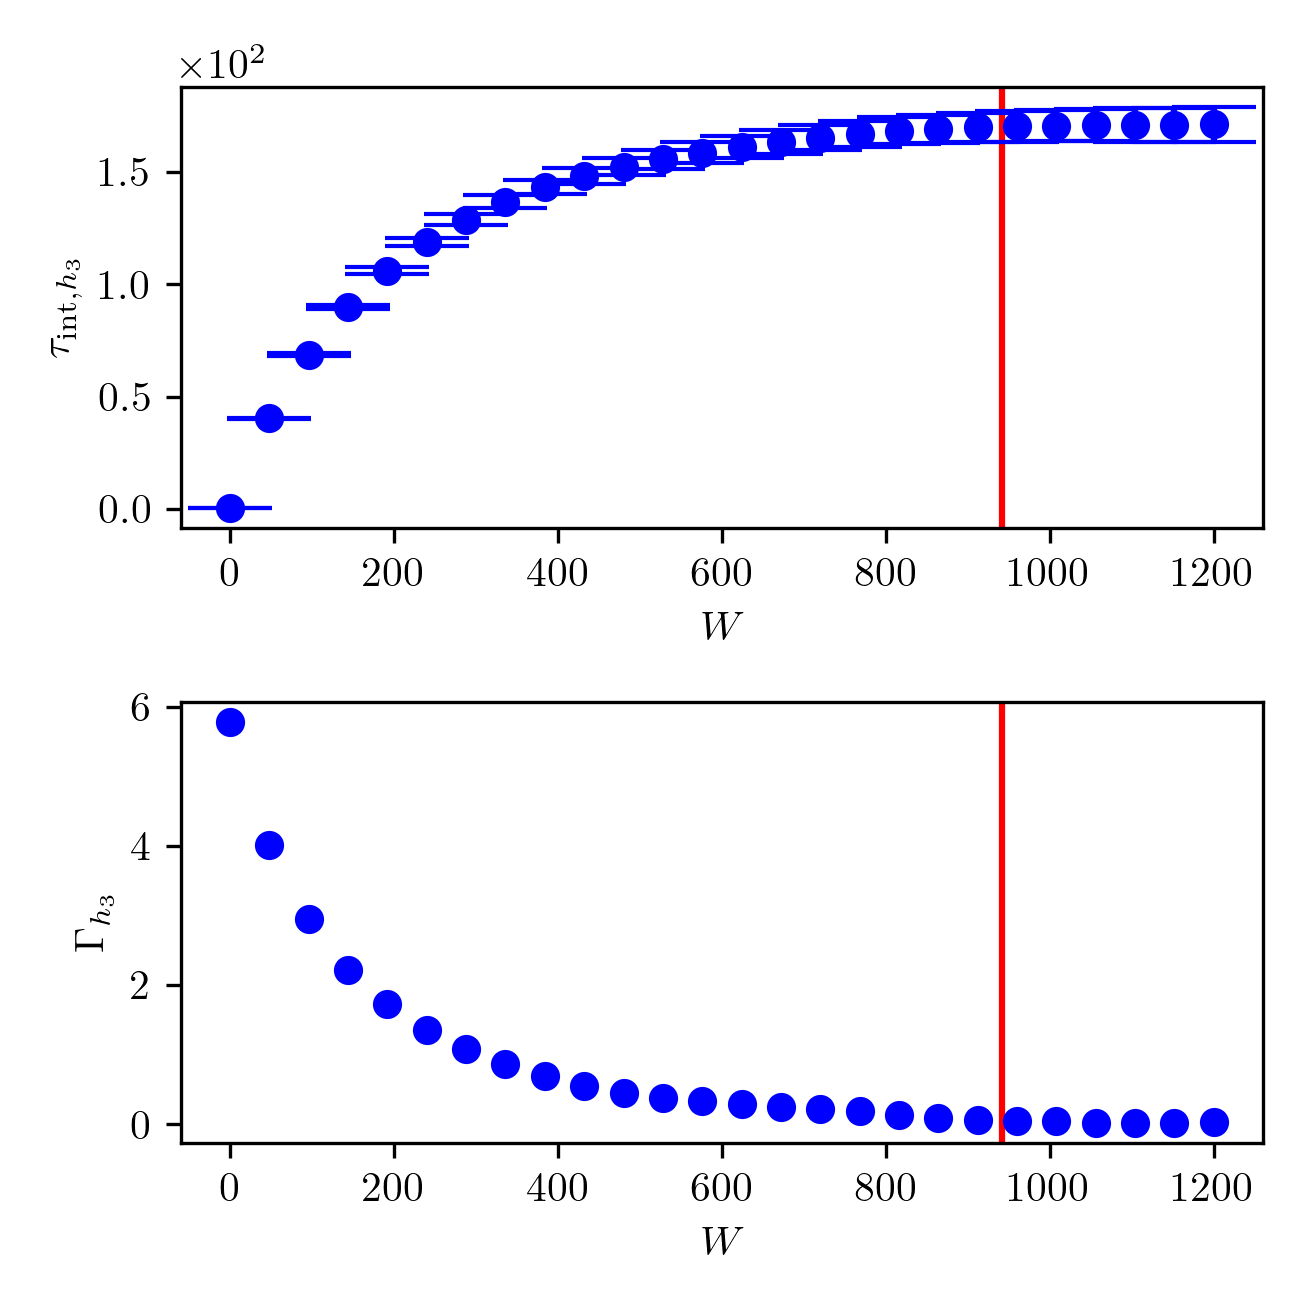
\includegraphics{UwerrTauIntTWalk2.png}
	\caption[]{}
	\label{fig:}
\end{figure}


\begin{figure}[ht!]
	\centering
	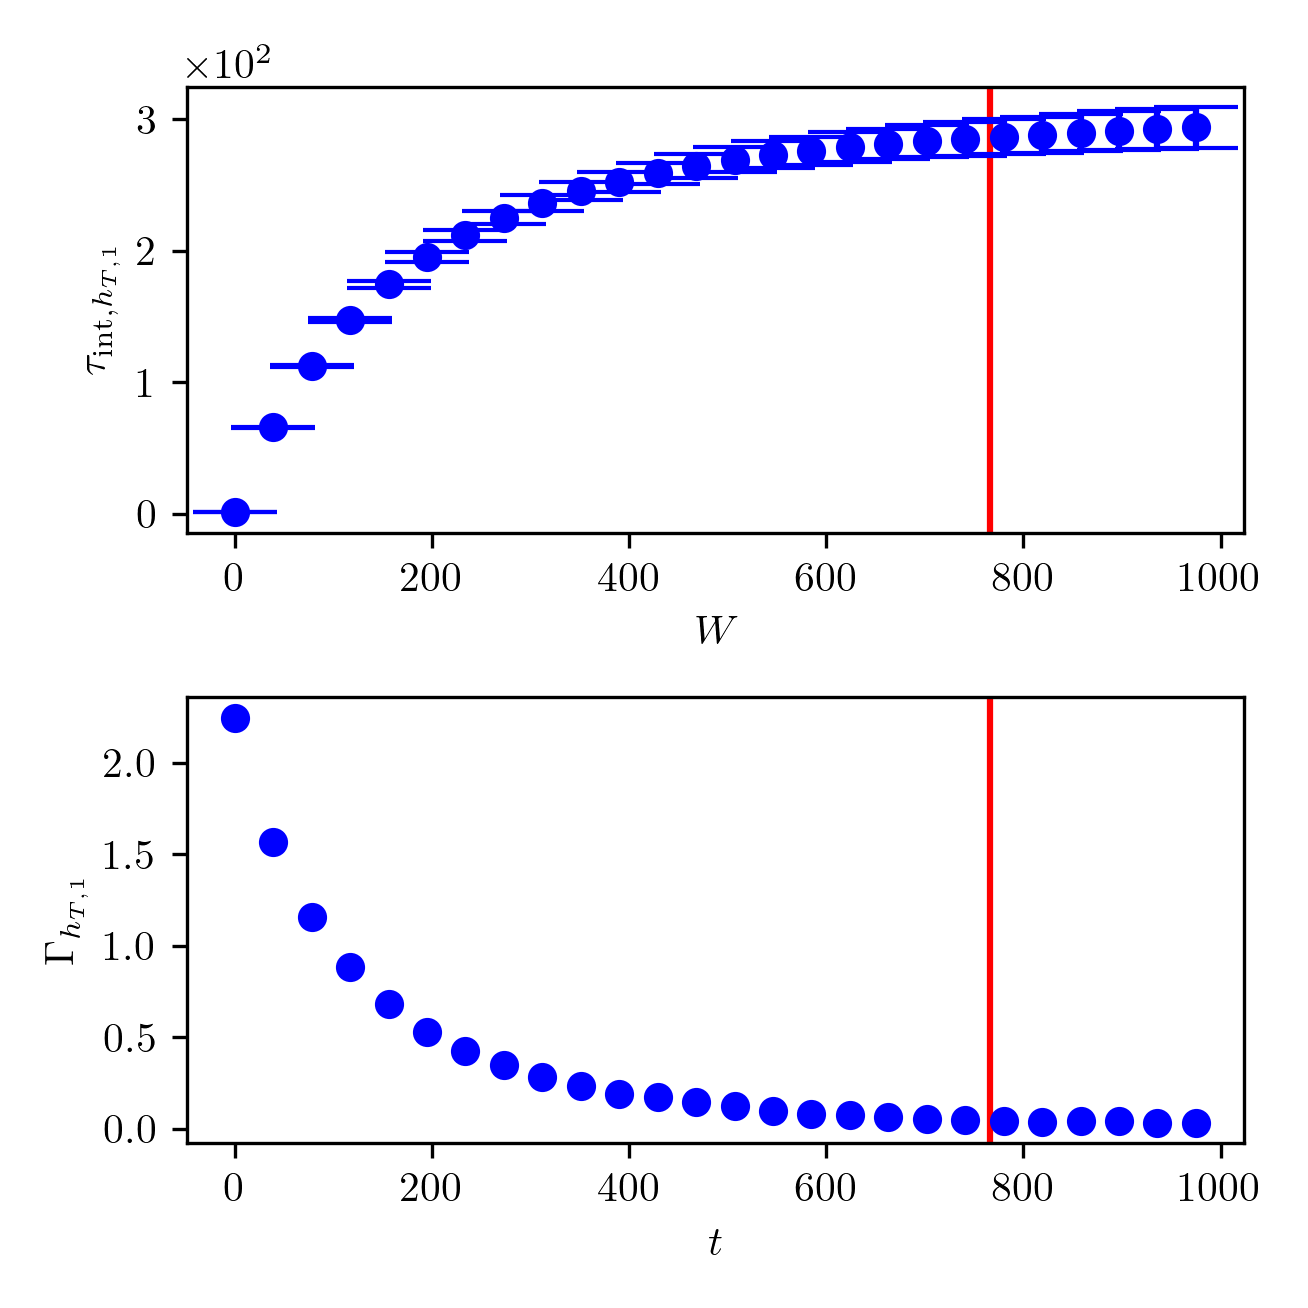
\includegraphics{UwerrTauIntTWalk3.png}
	\caption[]{}
	\label{fig:}
\end{figure}


\begin{figure}[ht!]
	\centering
	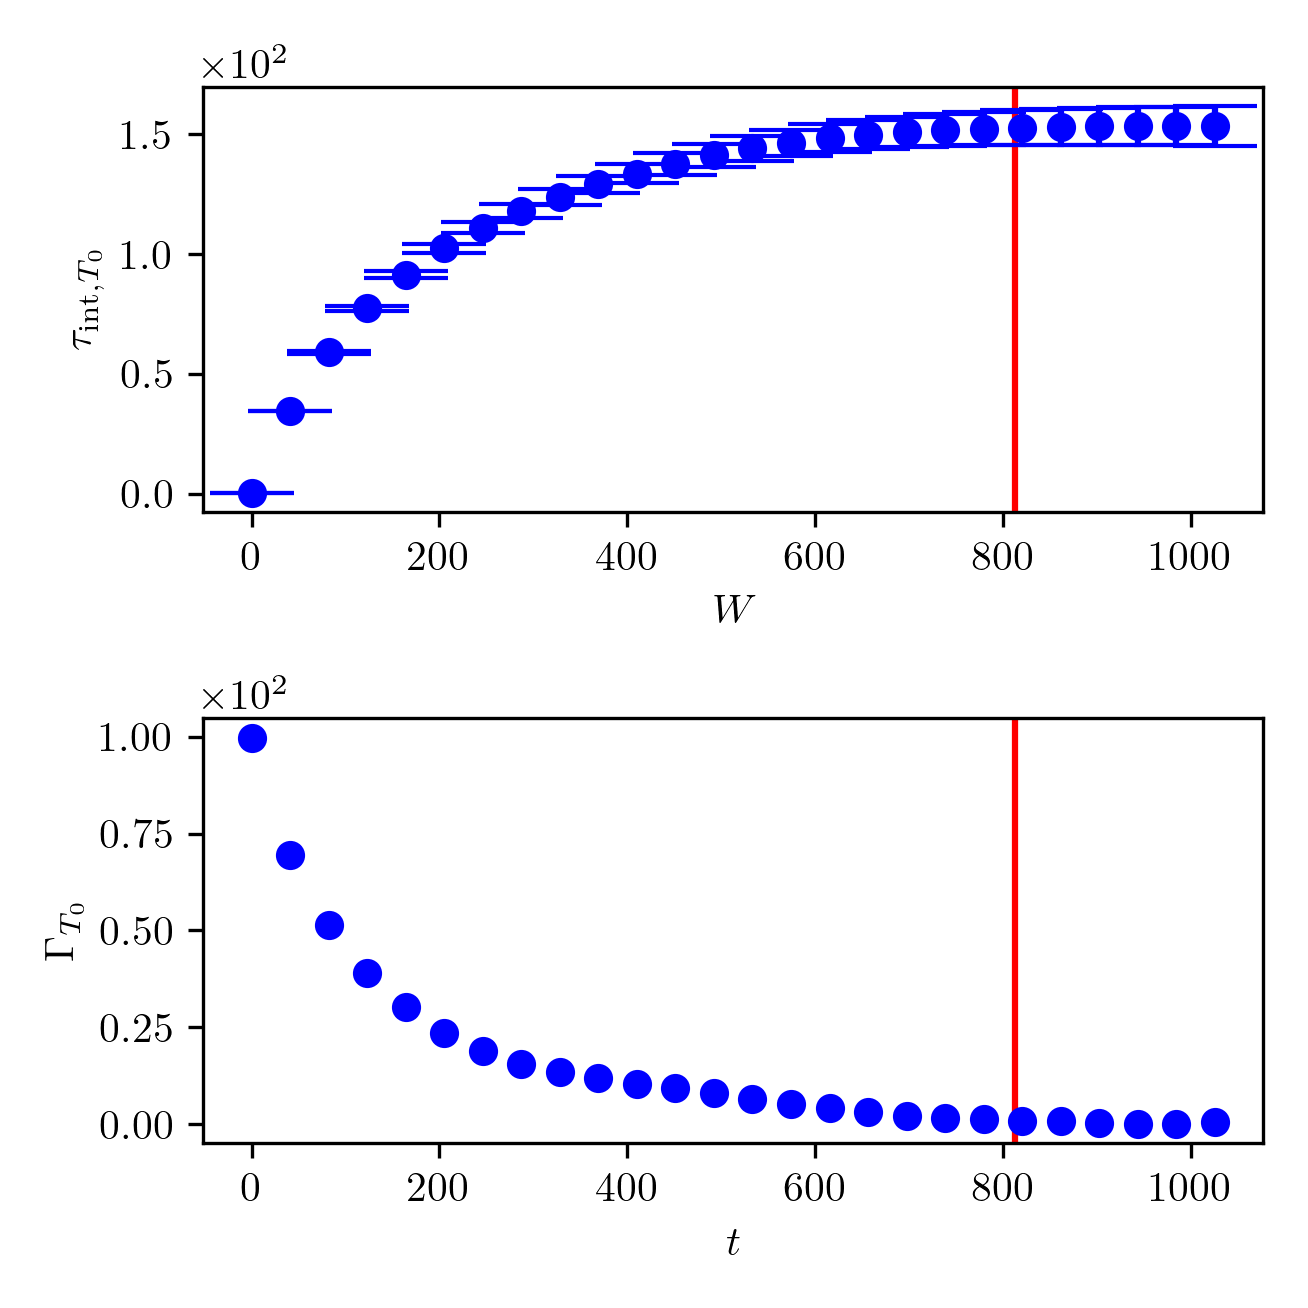
\includegraphics{UwerrTauIntTWalk4.png}
	\caption[]{}
	\label{fig:}
\end{figure}


\begin{figure}[ht!]
	\centering
	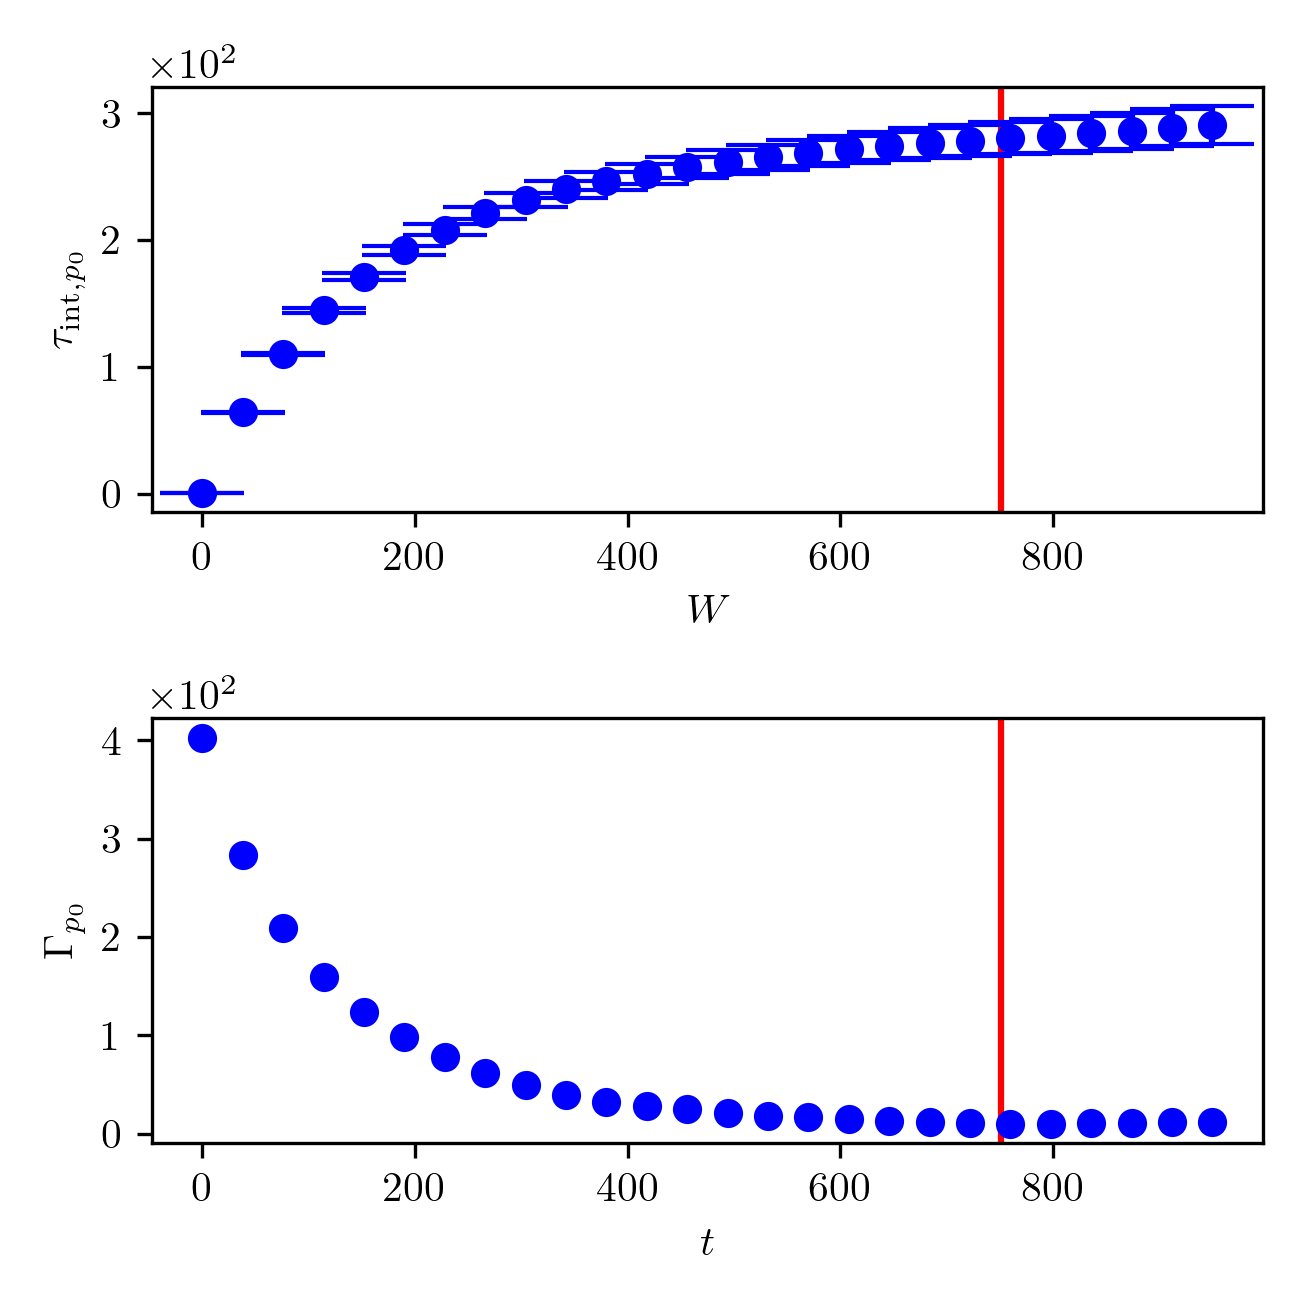
\includegraphics{UwerrTauIntTWalk5.png}
	\caption[]{}
	\label{fig:}
\end{figure}


\begin{figure}[ht!]
	\centering
	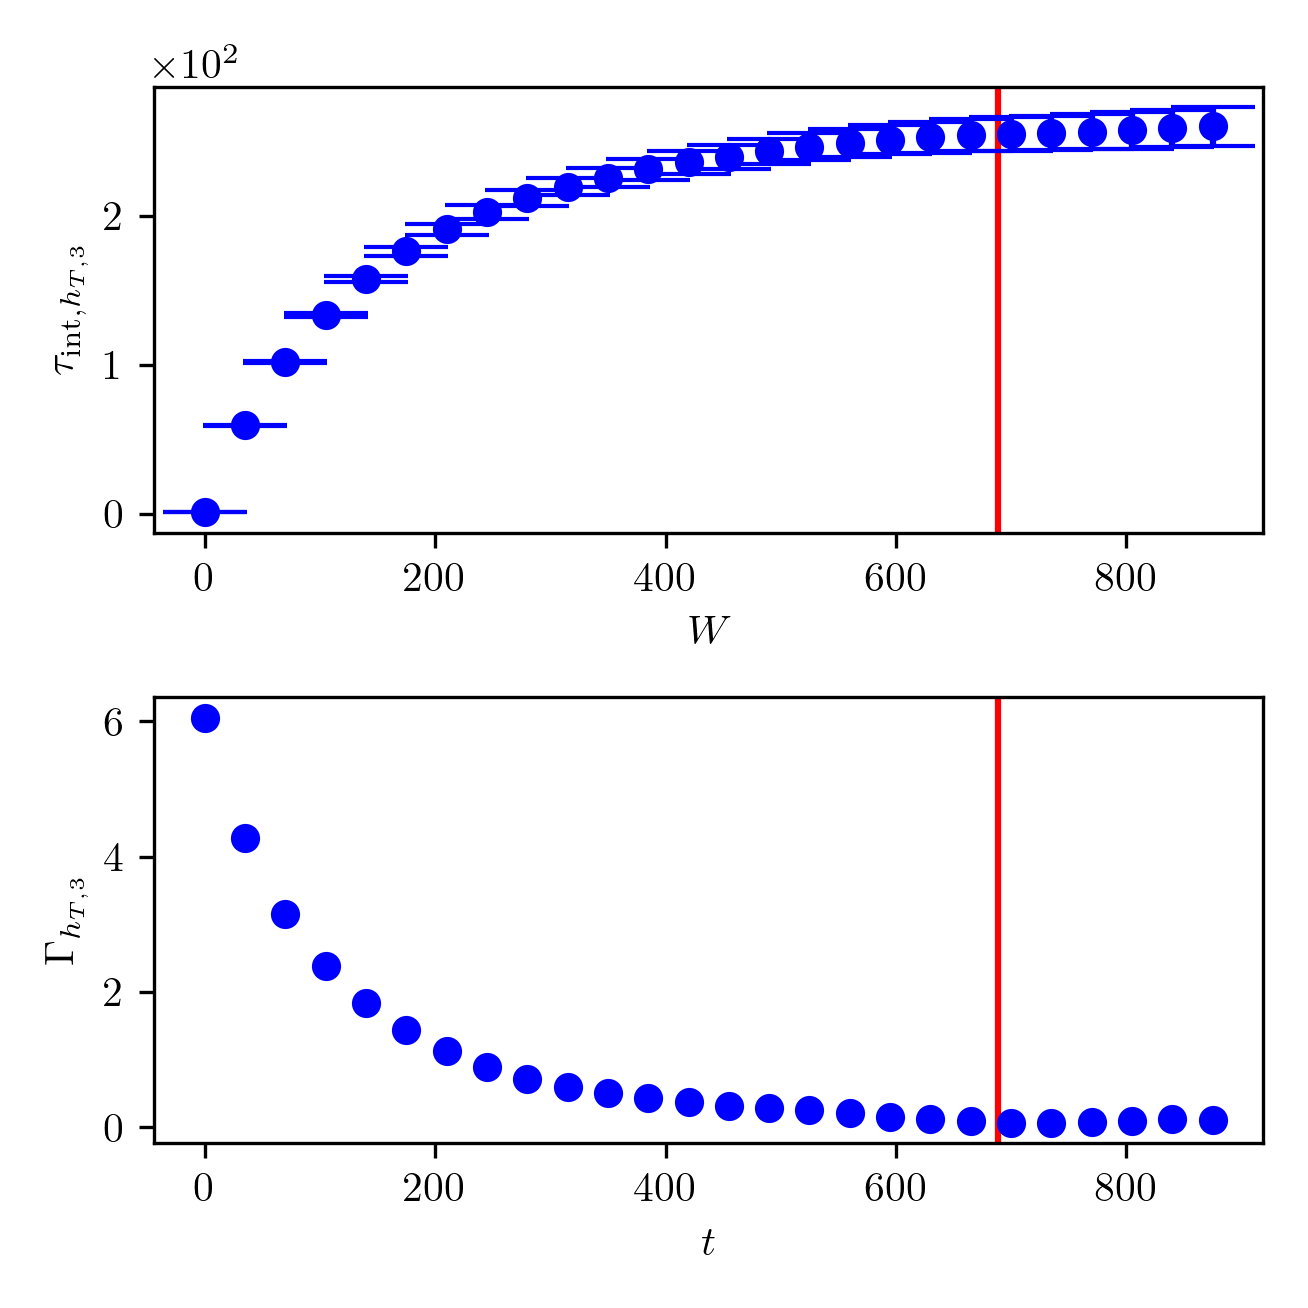
\includegraphics{UwerrTauIntTWalk6.png}
	\caption[]{}
	\label{fig:}
\end{figure}

\begin{figure}[ht!]
	\centering
	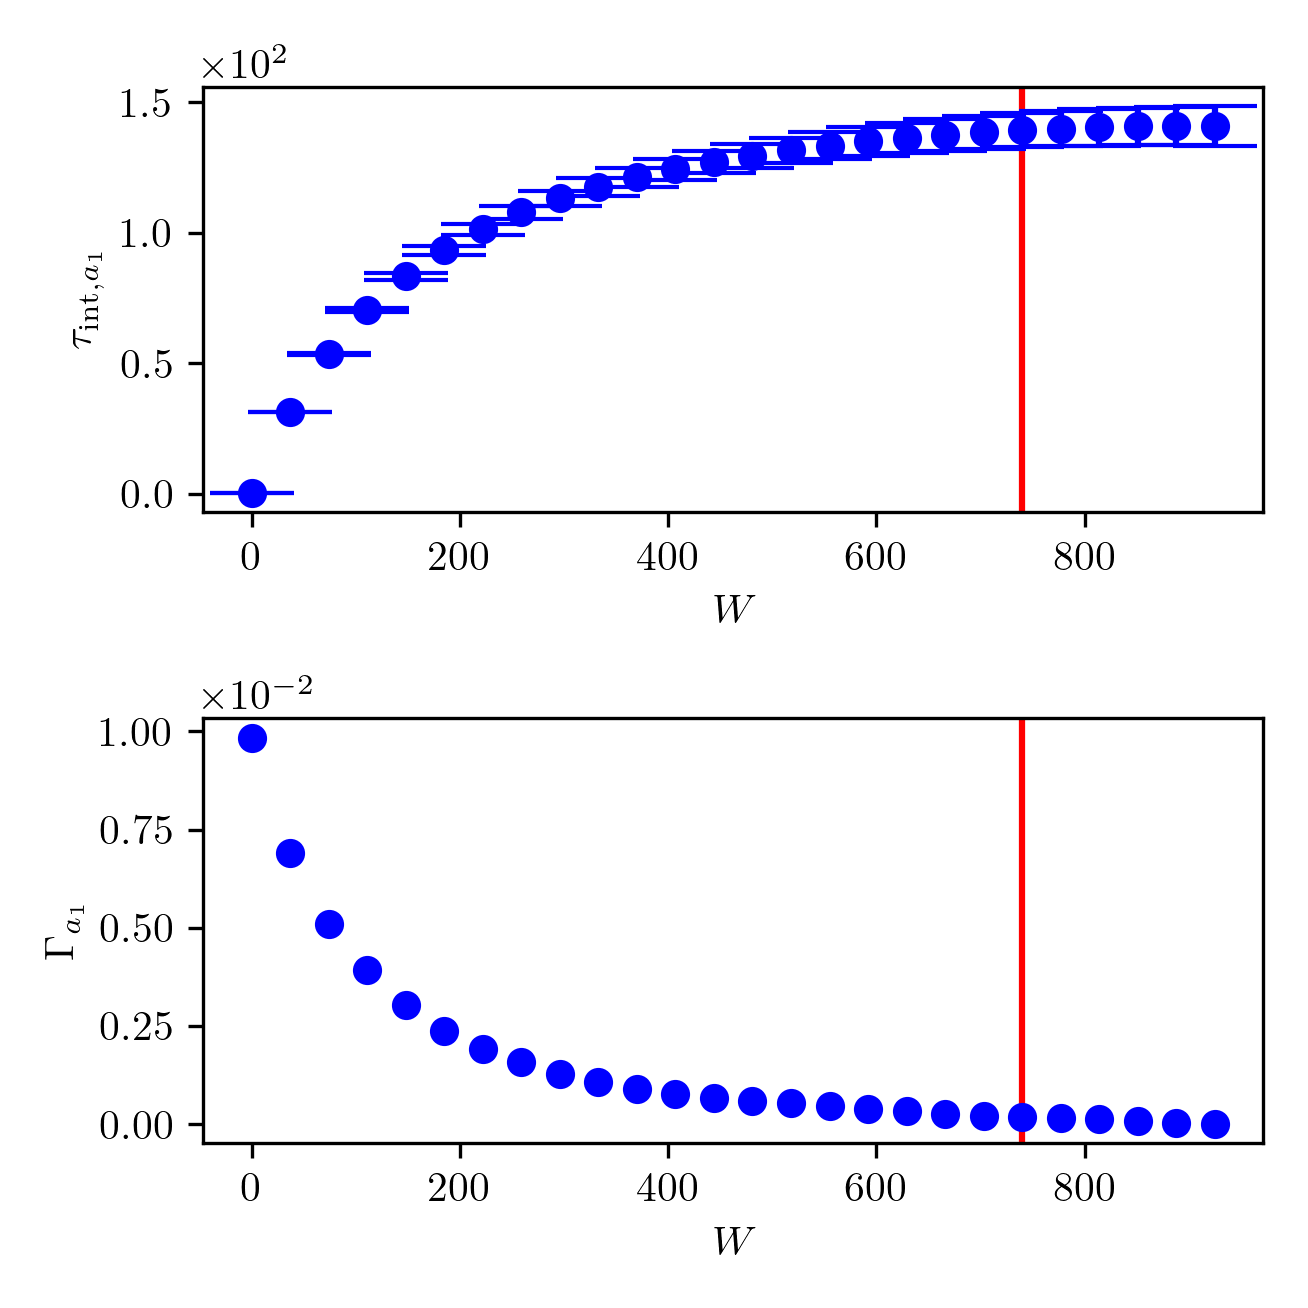
\includegraphics{UwerrTauIntTWalk7.png}
	\caption[]{}
	\label{fig:}
\end{figure}


\begin{figure}[ht!]
	\centering
	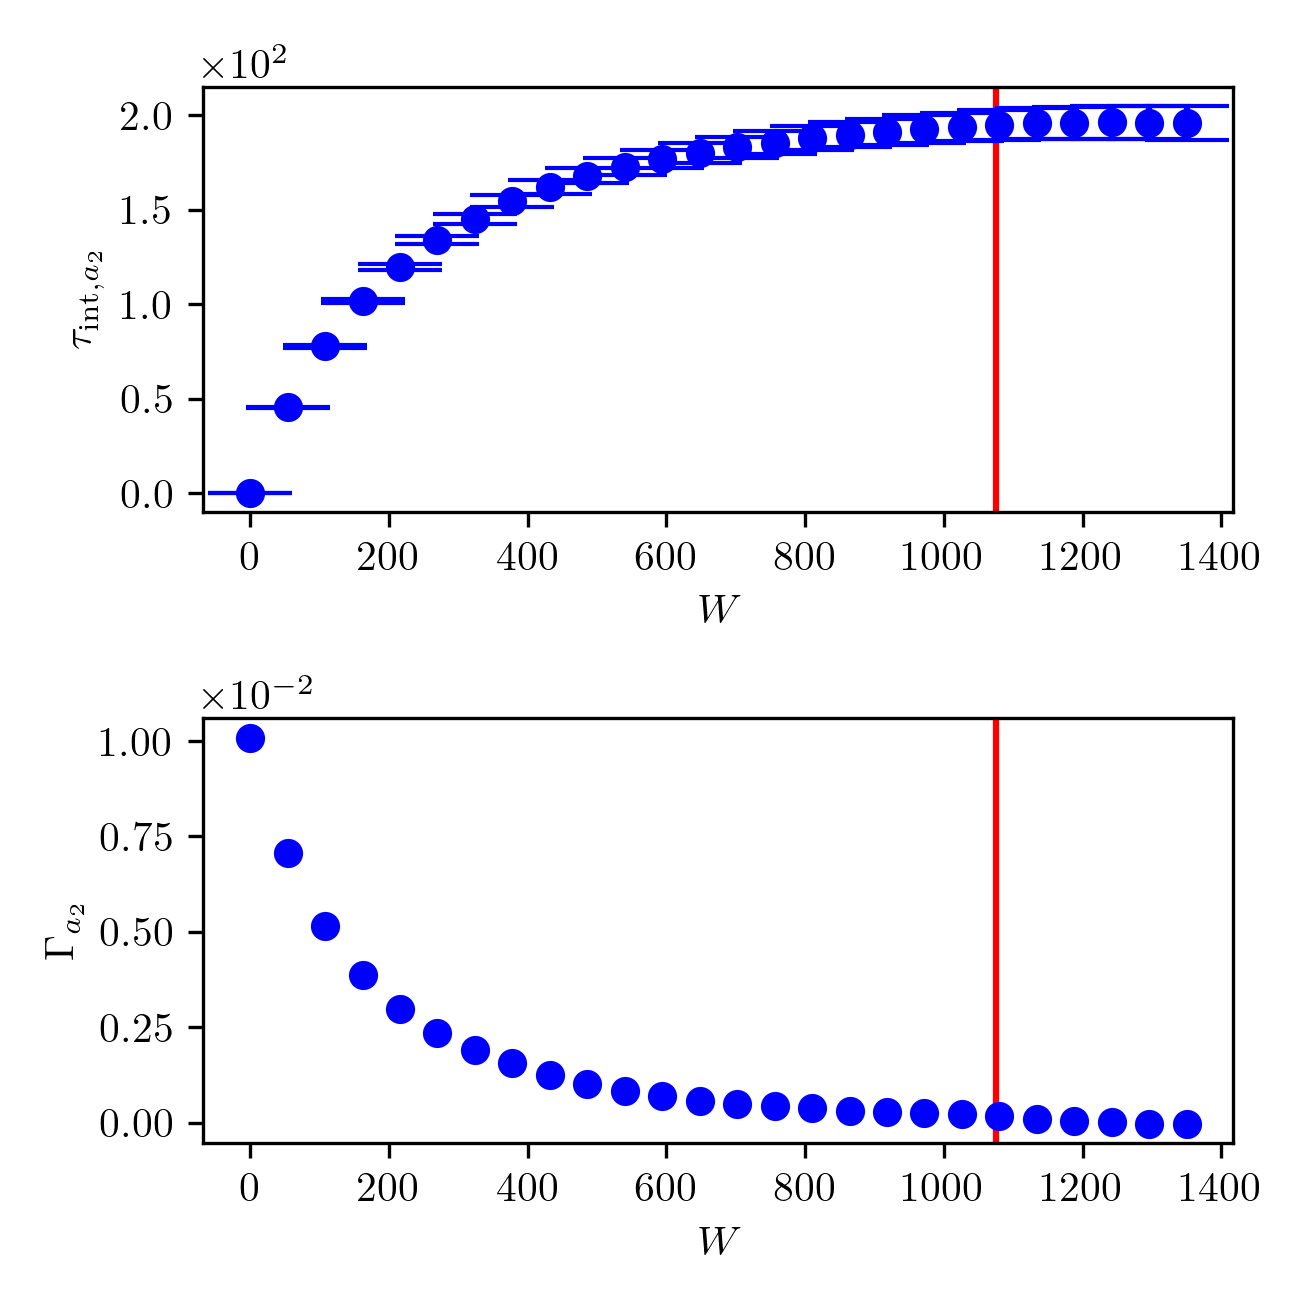
\includegraphics{UwerrTauIntTWalk8.png}
	\caption[]{}
	\label{fig:}
\end{figure}


\begin{figure}[ht!]
	\centering
	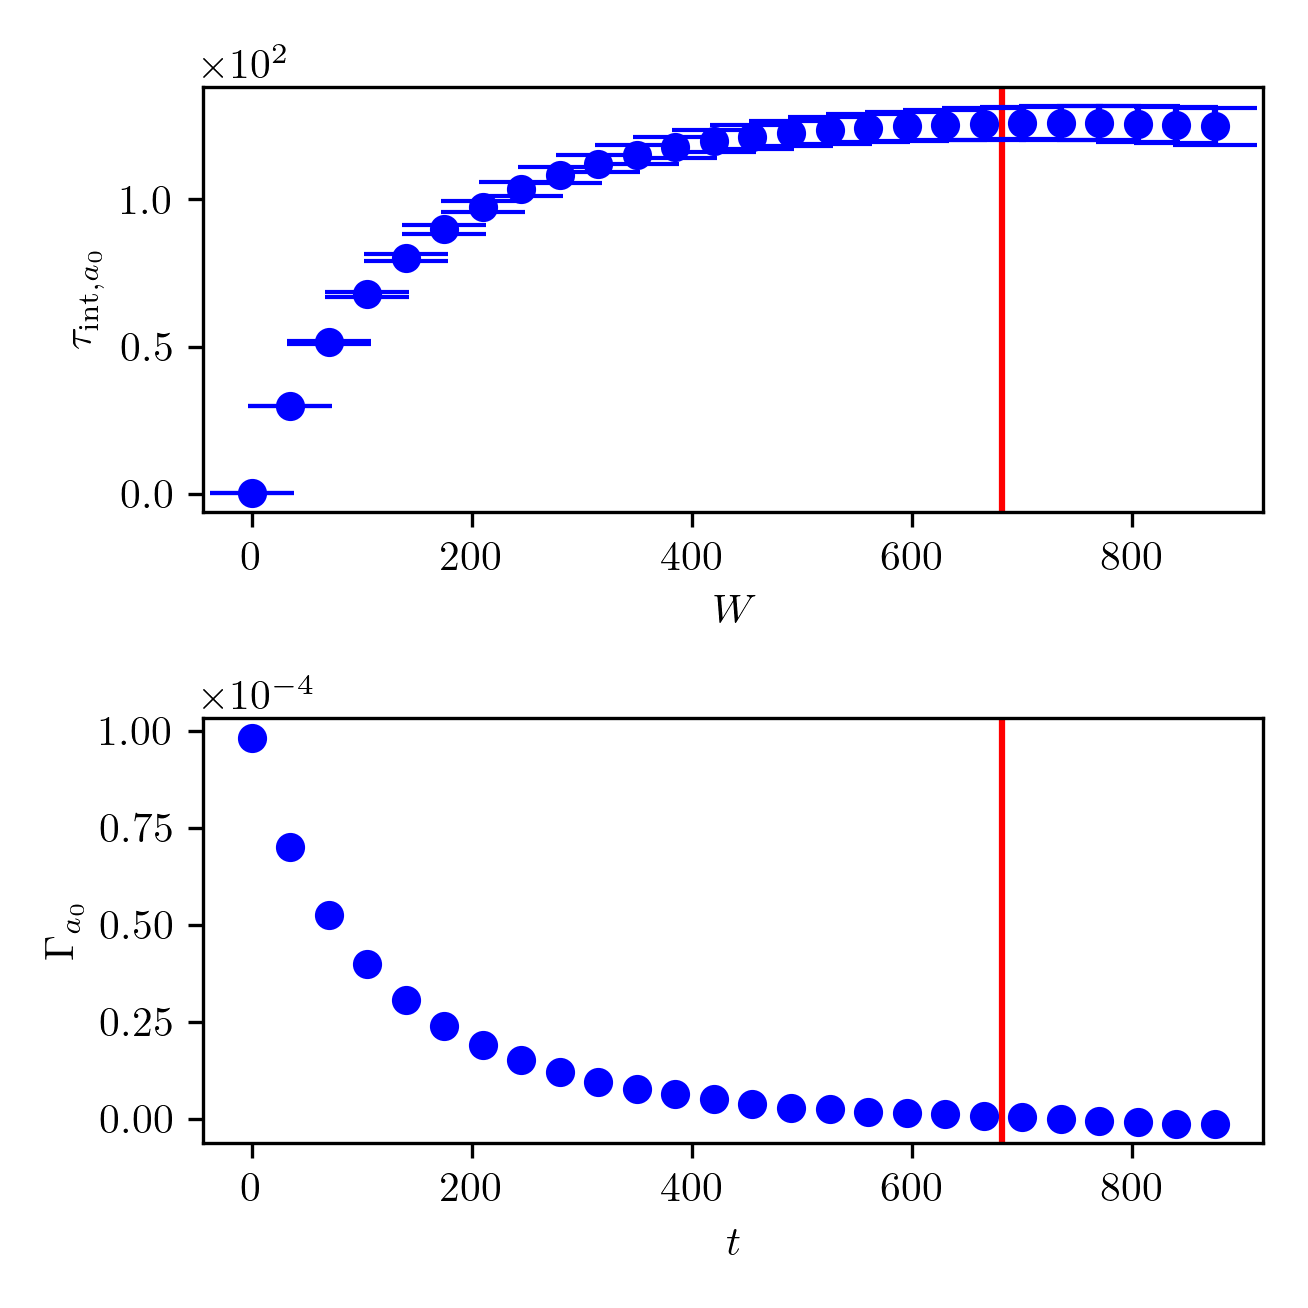
\includegraphics{UwerrTauIntTWalk9.png}
	\caption[]{}
	\label{fig:}
\end{figure}

\begin{figure}[ht!]
	\centering
	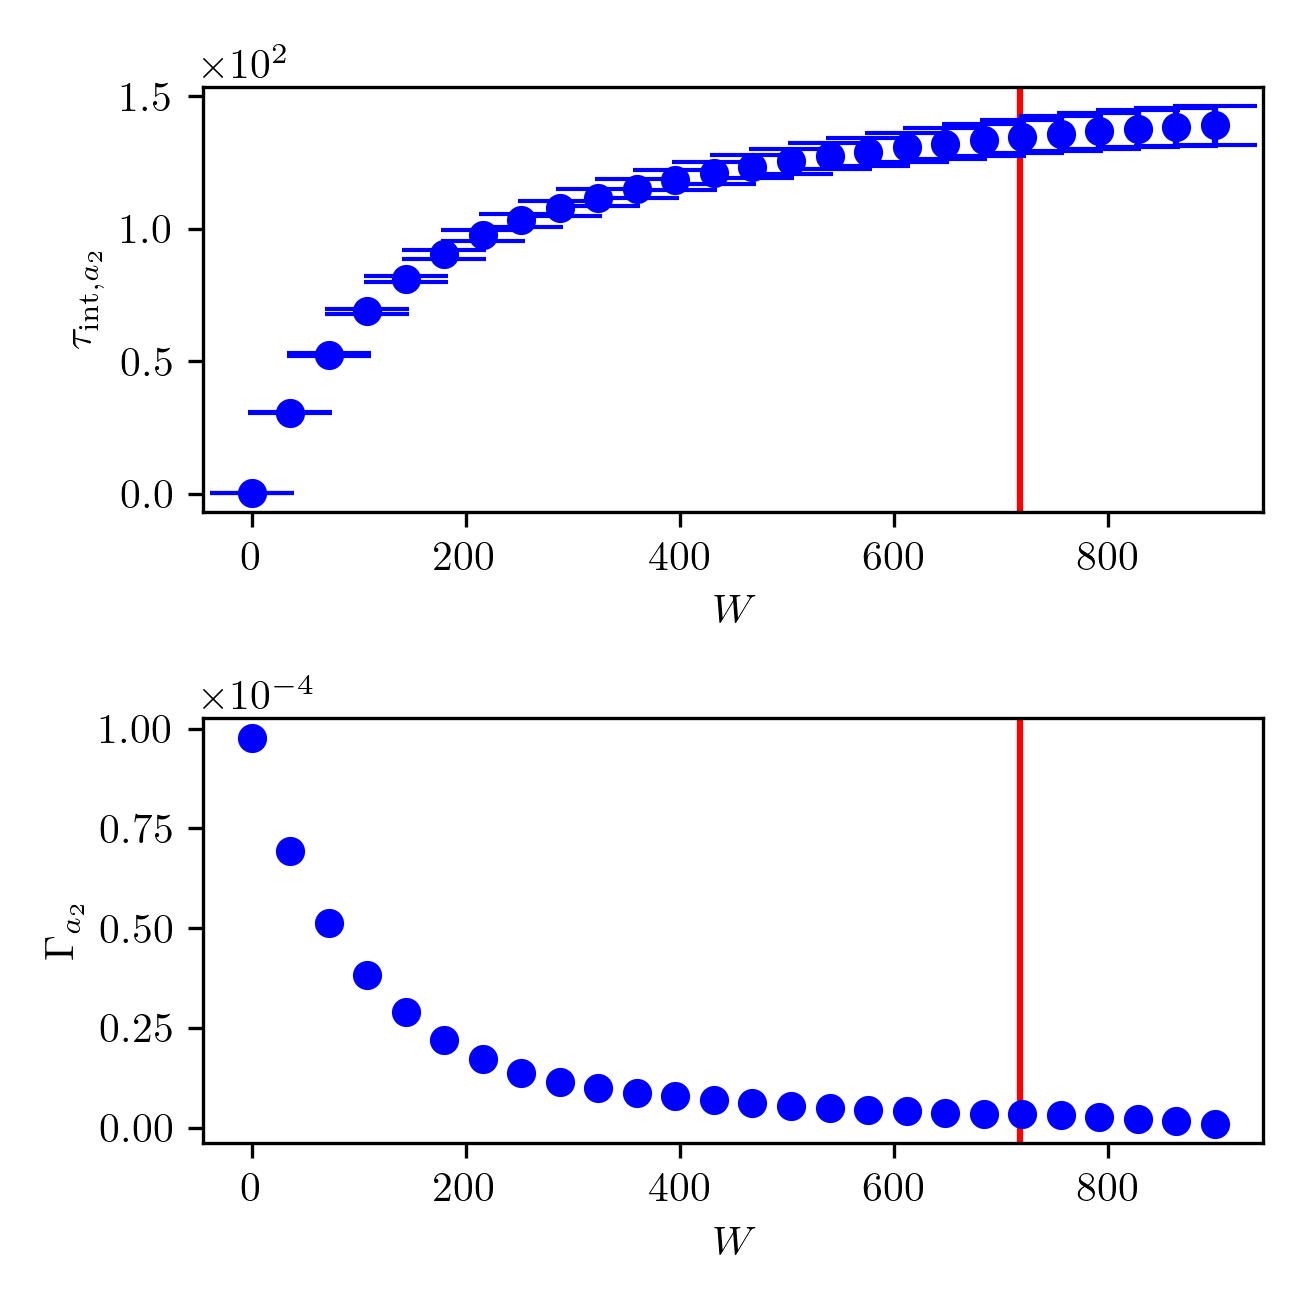
\includegraphics{UwerrTauIntTWalk10.png}
	\caption[]{}
	\label{fig:}
\end{figure}


\begin{figure}[ht!]
	\centering
	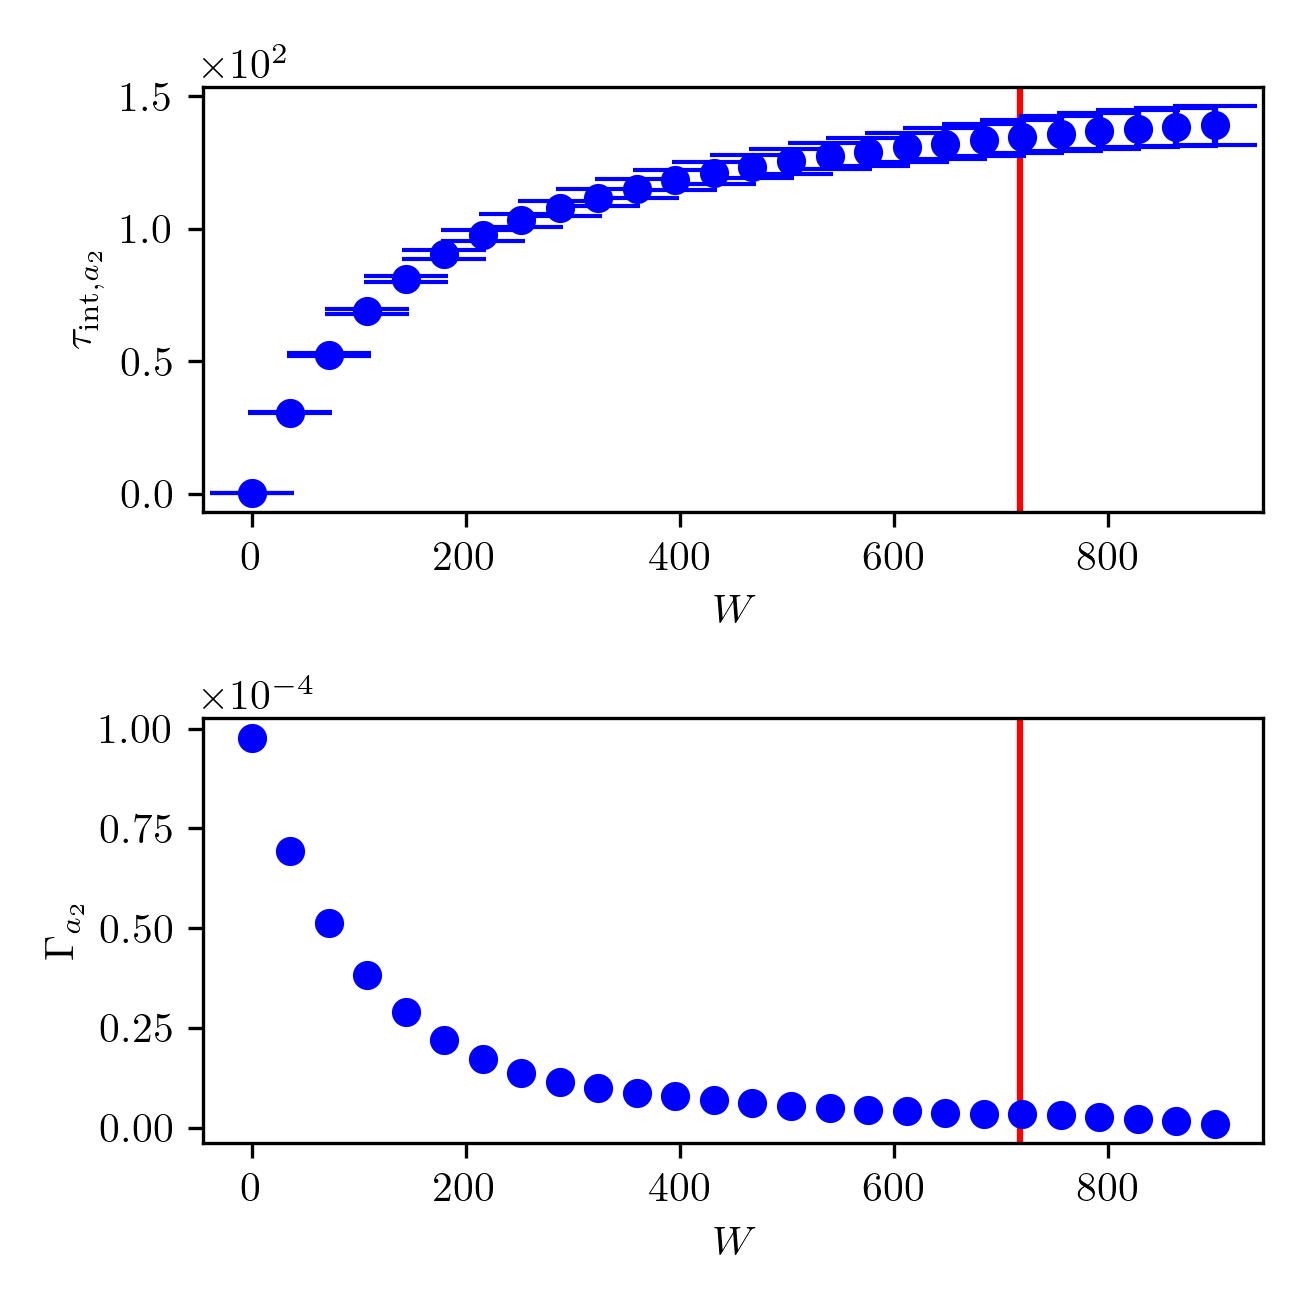
\includegraphics{UwerrTauIntTWalk10.png}
	\caption[]{}
	\label{fig:}
\end{figure}
\begin{figure}[ht!]
	\centering
	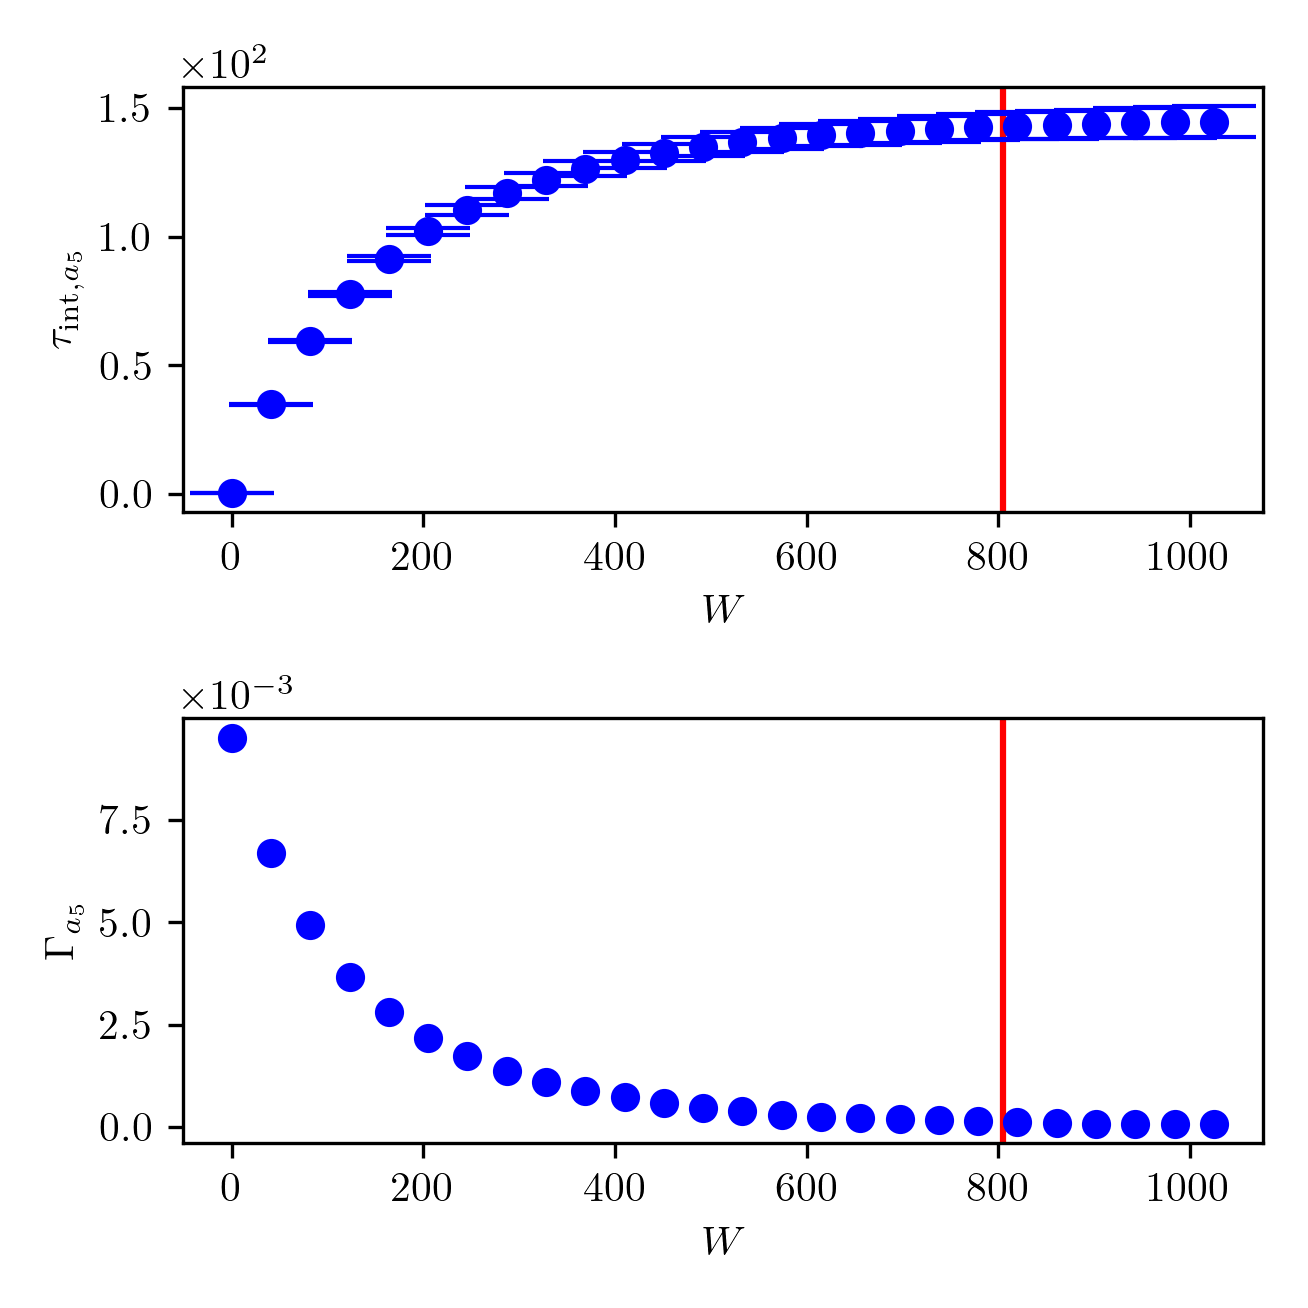
\includegraphics{UwerrTauIntTWalk11.png}
	\caption[]{}
	\label{fig:}
\end{figure}
\begin{figure}[ht!]
	\centering
	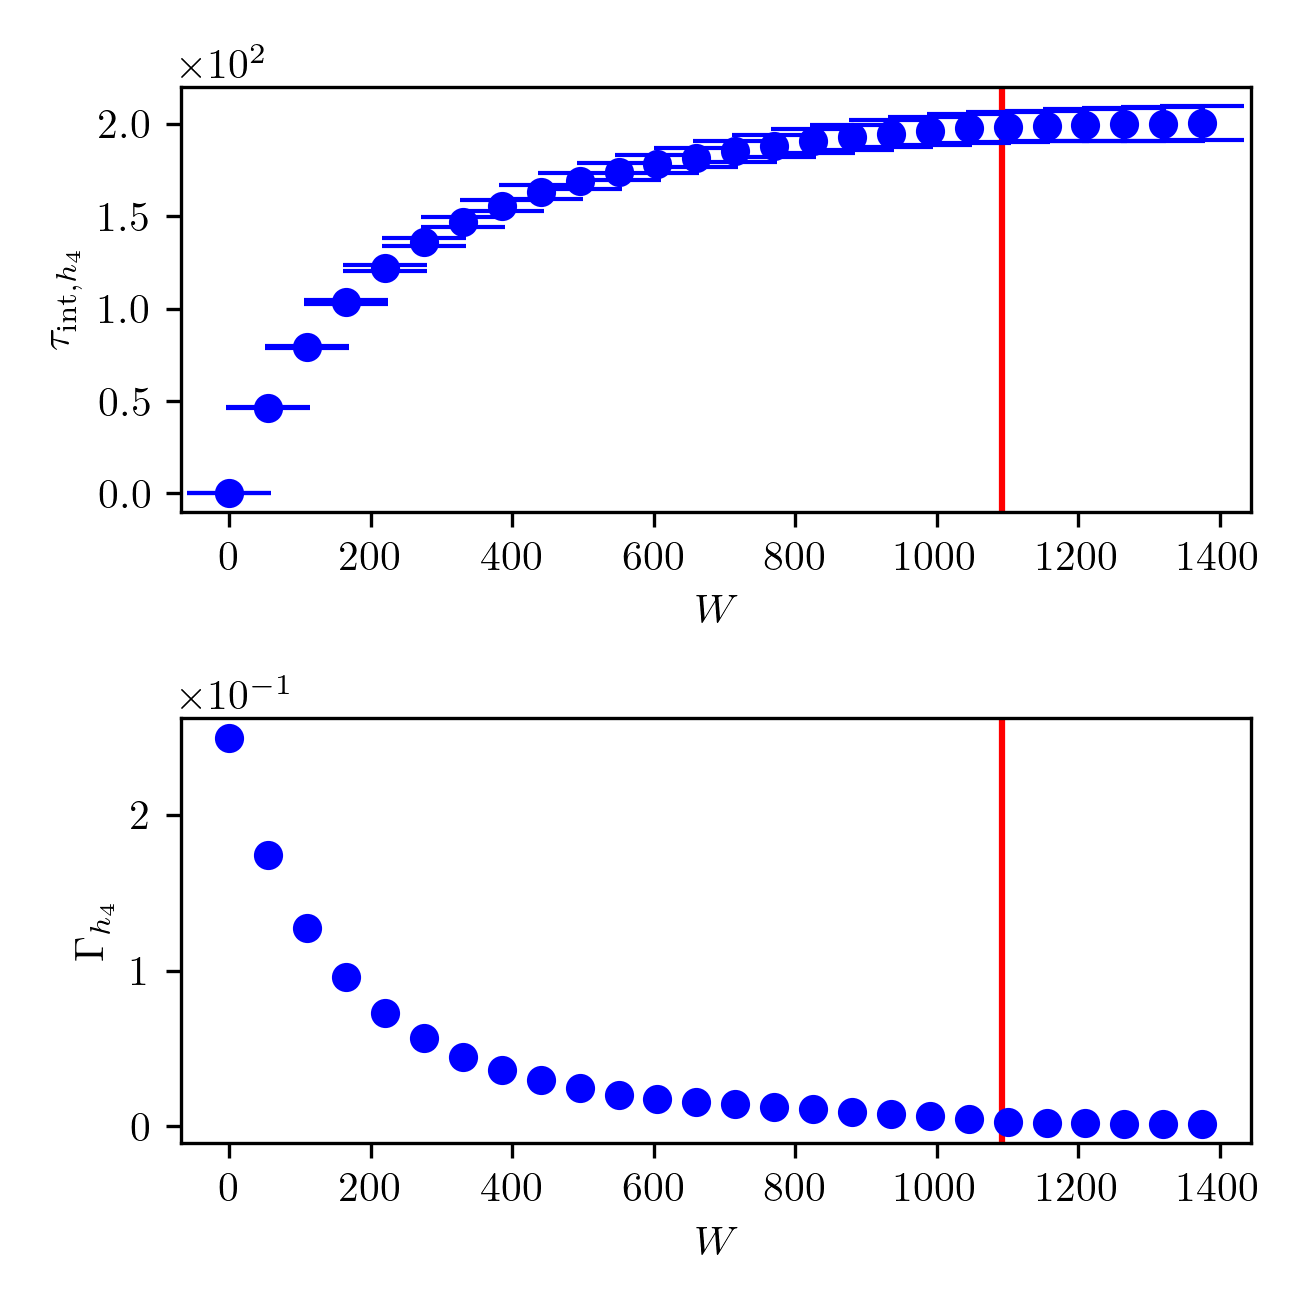
\includegraphics{UwerrTauIntTWalk12.png}
	\caption[]{}
	\label{fig:}
\end{figure}
\begin{figure}[ht!]
\centering
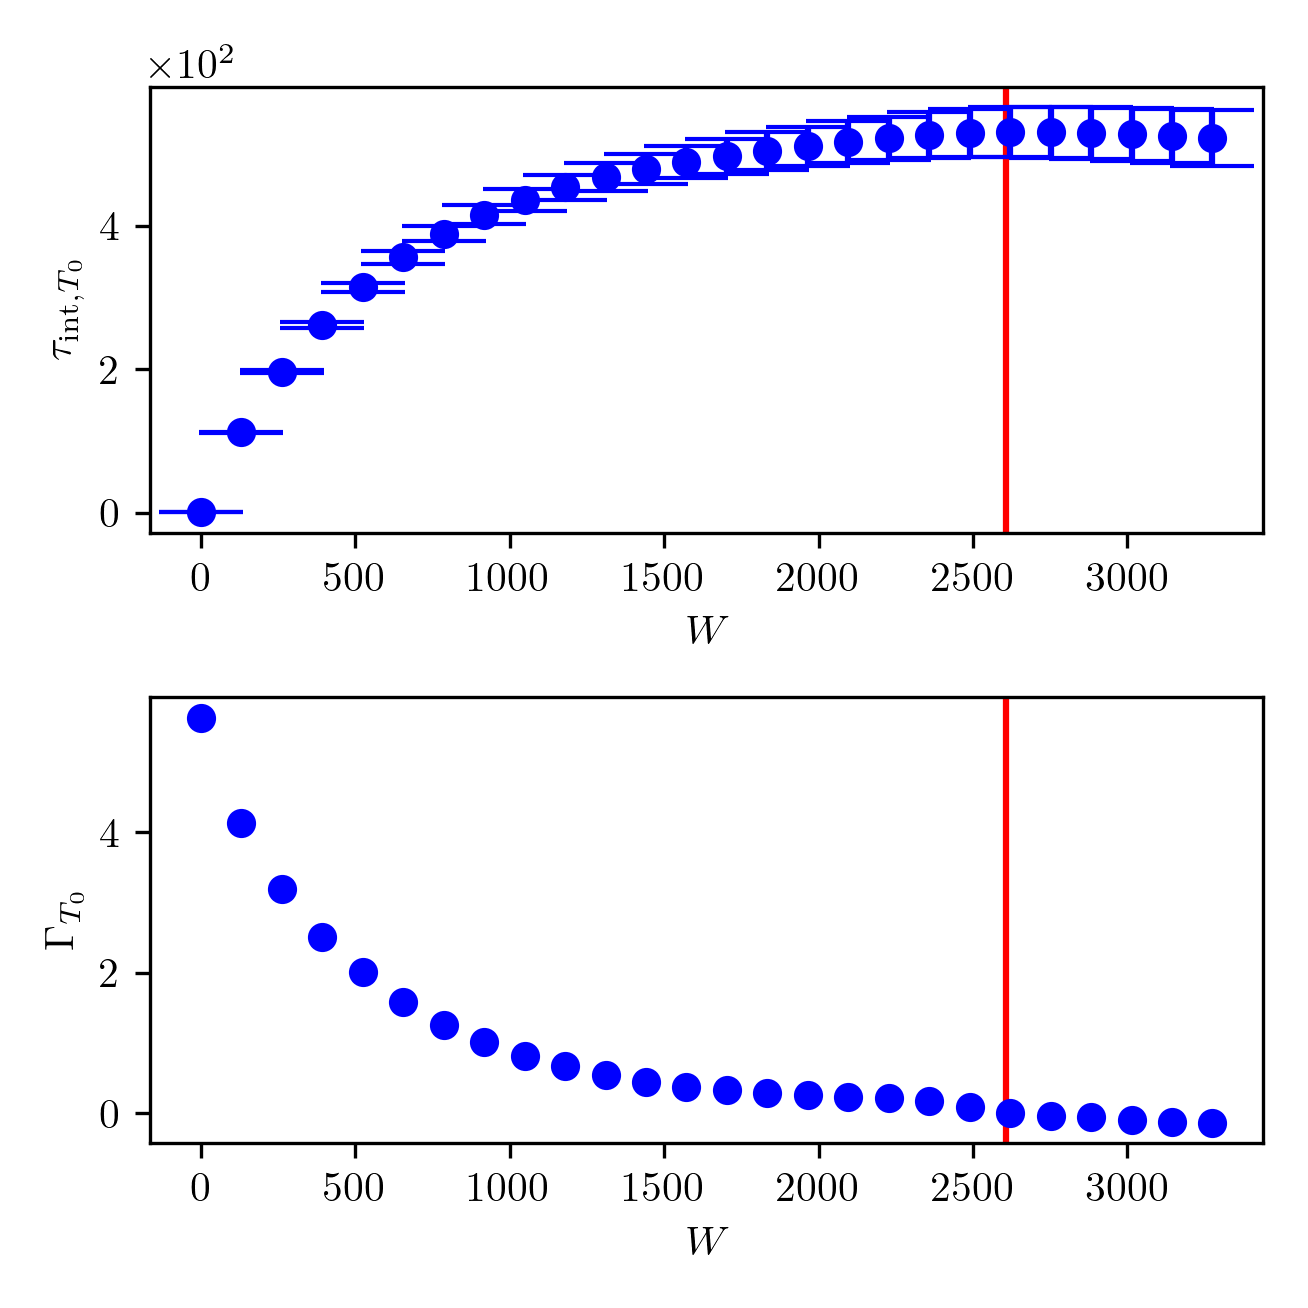
\includegraphics{UwerrTauIntTWalk13.png}
\caption[]{}
\label{fig:}
\end{figure}
\begin{figure}[ht!]
	\centering
	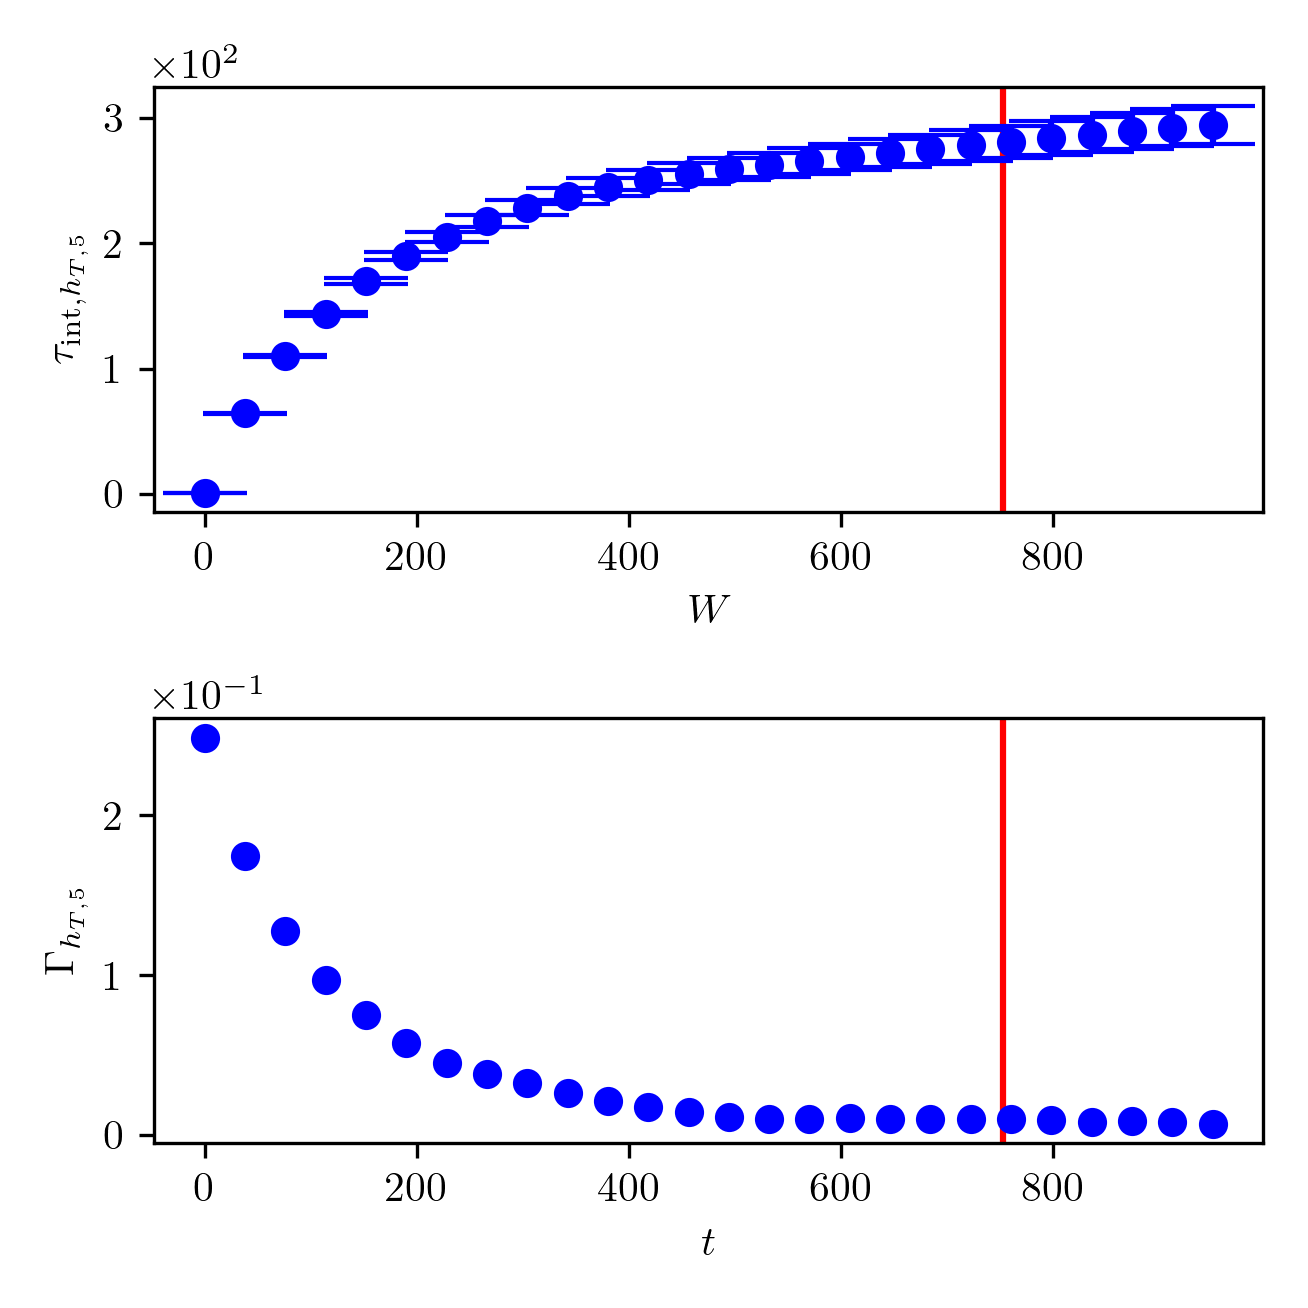
\includegraphics{UwerrTauIntTWalk14.png}
	\caption[]{}
	\label{fig:}
\end{figure}

\begin{figure}[ht!]
	\centering
	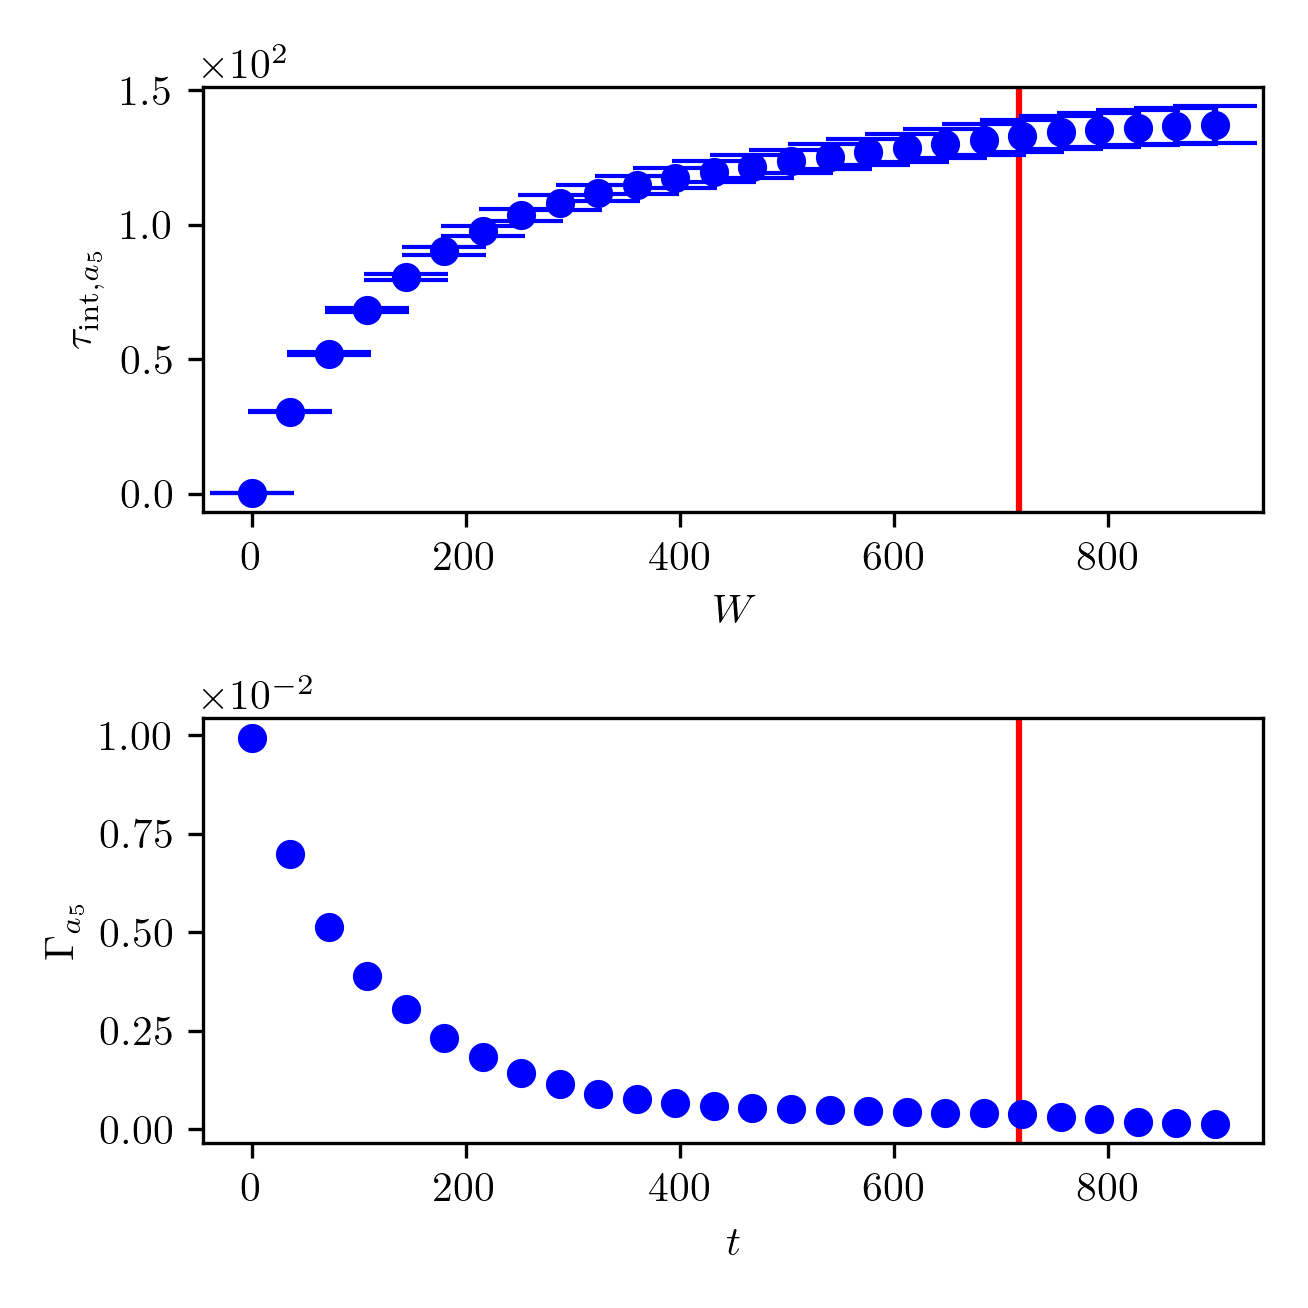
\includegraphics{UwerrTauIntTWalk15.png}
	\caption[]{}
	\label{fig:}
\end{figure}



\section{Ozone}
\begin{figure}[htb!]
	\centering
	\begin{tikzpicture}
		\node[roundnode2] at (-4,6.5) (Q)     {$\bm{Q}$};
		\node[roundnode2] at (-2.5,5) (x)     {$\bm{x}$};
		\node[align=center] at (-1,4) (A)    {$\bm{A}$};
		\node[roundnode2] at (-1,2.5) (u)    {$\bm{\Omega}$};
		\node[rectnode] at (-1,1) (y)    {$\bm{y}$};
		\node[roundnode2] at (-2.5,2.5) (e)    {$\bm{\eta}$};
		\node[roundnode2] at (-6.5,6.5) (S)    {$\bm{\Sigma}$};
		\node[roundnode2] at (-8,8) (s)    {$\gamma$};
		\node[roundnode2] at (-5.5,8) (d)    {$\delta$};
		
		%Lines
		\draw[->, very thick] (S) -- (e);
		\draw[->, mydotted, very thick] (s) -- (S);
		\draw[->, mydotted, very thick] (e) -- (y);
		\draw[->, very thick] (u.south) -- (y);
		\draw[->, mydotted, very thick] (A) -- (u);
		\draw[->, mydotted,  very thick] (x) -- (A.west);
		
		\draw[->, mydotted, very thick] (d) -- (Q); 
		
		\draw[->, very thick] (Q) -- (x); 
		%\node[align=center] at (0,4) (f3) {$= \bm{A}$};
		%\node[align=center] at (0.25,3.95) (f3) {$\approx \bm{M A}_L$};
		\node[align =center] at (-1,7) (T1) {marginal posterior \\ over hyper-parameters \\ $\pi(\gamma, \delta | \bm{y})$};
		\node[align =center] at (0,5) (T1) {conditional posterior \\ $\pi( \bm{x} |\gamma, \delta, \bm{y})$ };
		
		
		\node[fit=(S)(s)(Q)(d),draw,dotted,black, rounded corners] {};
	\end{tikzpicture} 
	\caption[Directed acyclic graph for ozone retrieval and MTC scheme.]{Directed acyclic graph for modelling and measuring process of ozone highlighting the marginal and then conditional (MTC) scheme. The hyper-parameters $\delta$ and $\gamma$ determine the noise covariance $\bm{\Sigma} = \gamma^{-1}\bm{I}$ for the random noise vector $\bm{\eta} \sim \mathcal{N}(0, \gamma^{-1}\bm{I})$ and the prior precision matrix $\bm{Q} = \delta \bm{L}$ for the normal distribution over $\bm{x} \sim \mathcal{N}(0, \delta \bm{L})$, where $\bm{L}$ is a graph Laplacian, see Eq. \ref{eq:GLapl}. In the MTC scheme we evaluate the marginal posterior over the hyper-parameters $\pi(\gamma, \delta | \bm{y})$ as in Eq. \ref{eq:} first and then the conditional posterior $\pi(\bm{x}|\gamma,\delta,\bm{y})$ as in Eq. \ref{eq:CondPost}. The MTC scheme allows to evaluate the marginal posterior distribution over the hyper-parameters $\delta, \gamma$ independent of $\bm{x}$, breaking the correlation structure.
	Through the forward model $\bm{A}_{NL} \approx \bm{M}\bm{A}_L$ and the parameter $\bm{x}$ we generate a space of all measurable from which we randomly observe a data set $\bm{y}$ including random noise $\bm{\eta}$.}
	\label{fig:DAGO3}
\end{figure}
\begin{figure}[ht!]
	\centering
	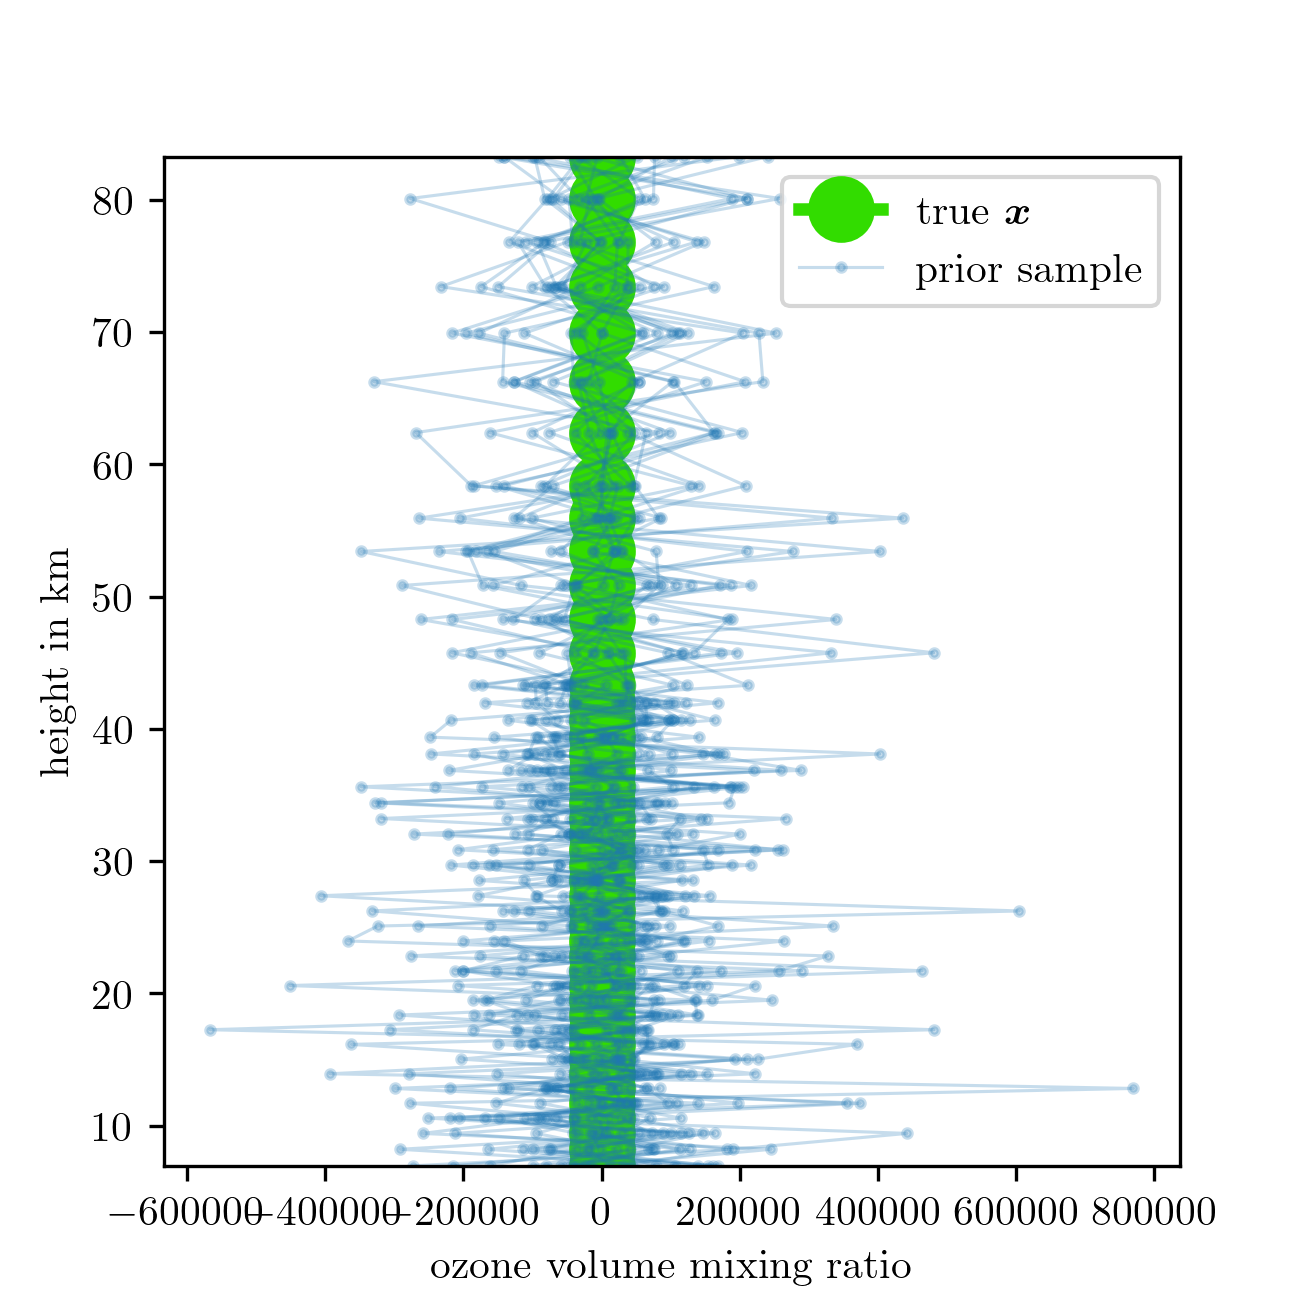
\includegraphics{OzonePrior.png}
	\caption[Samples from ozone prior distribution.]{We draw samples from ozone prior distribution $\bm{x} \sim \mathcal{N}(0,\delta \bm{L})$ after generating a sample from the hyper-prior distribution $\delta \sim \mathcal{T}(1,10^{-10})$. Note that since the variance of prior samples is very large compared to the ozone volume mixing ratios, the ozone profile appears to be constant, which is not the case, see e.g. Fig. \ref{fig:O3Samp}.}
	\label{fig:O3Prior}
\end{figure}


\clearpage
\section{Pressure over Temperature}
\begin{figure}[ht!]
	\centering
	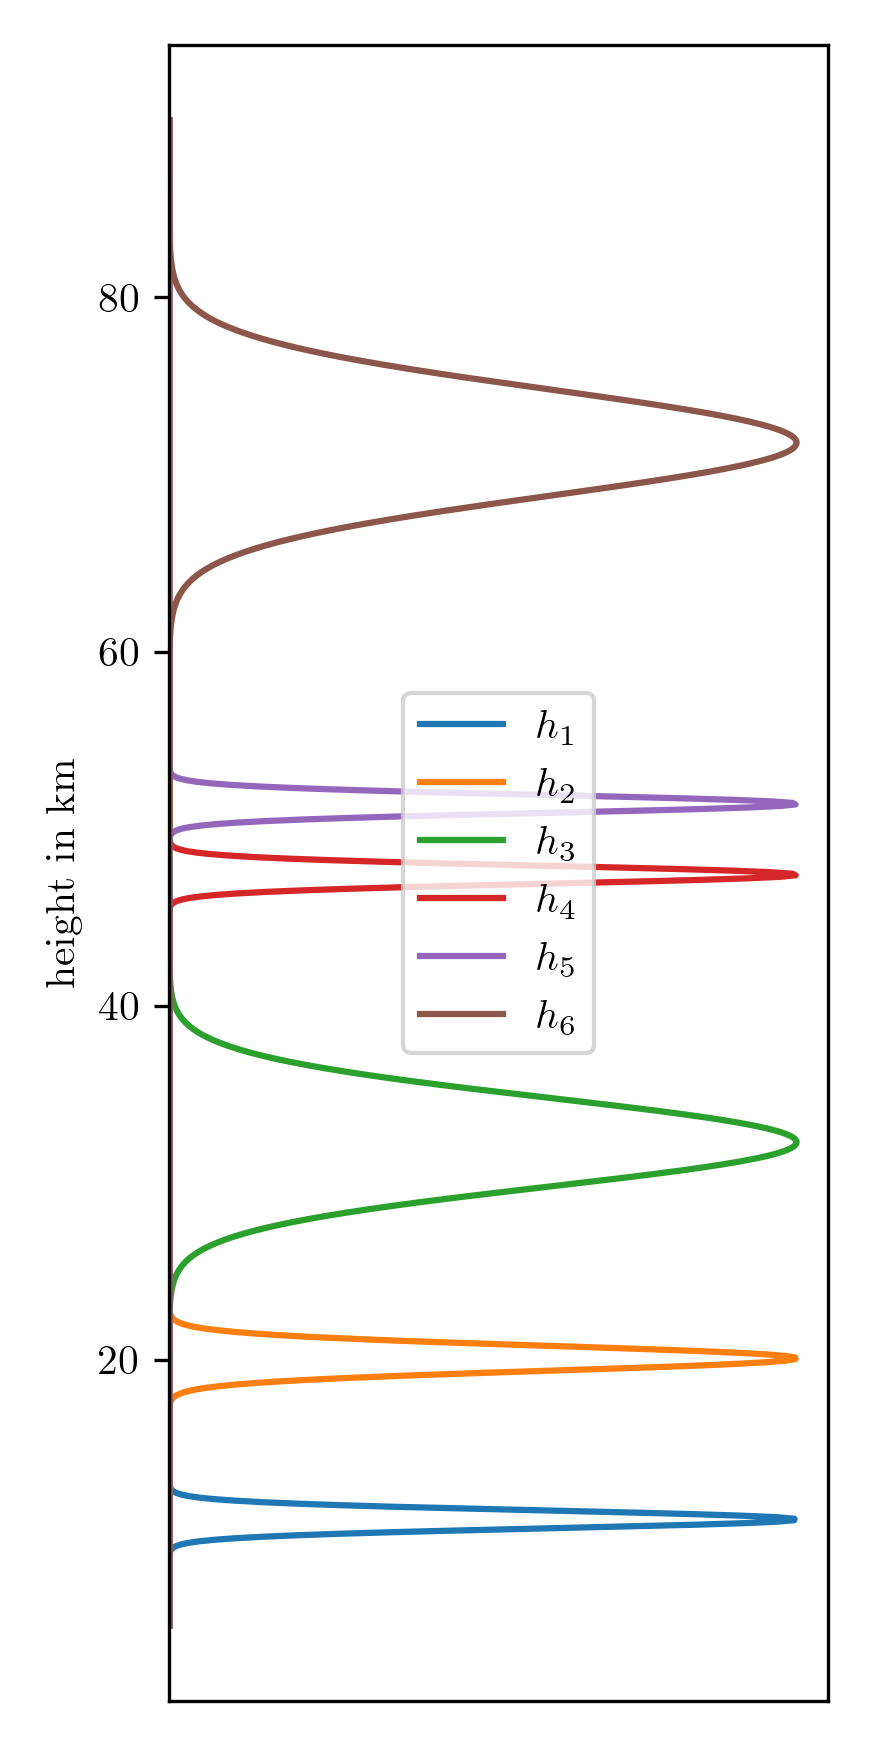
\includegraphics{HeightPriors.png}
	\caption[Prior distributions $\pi(h_T)$.]{Prior distributions $\pi(h_T)$, which we choose so that they do not overlap and not conflict with the temperature function \ref{eq:tempFunc}}
	\label{fig:HeightPriors}
\end{figure} 

\begin{figure}[ht!]
	\centering
	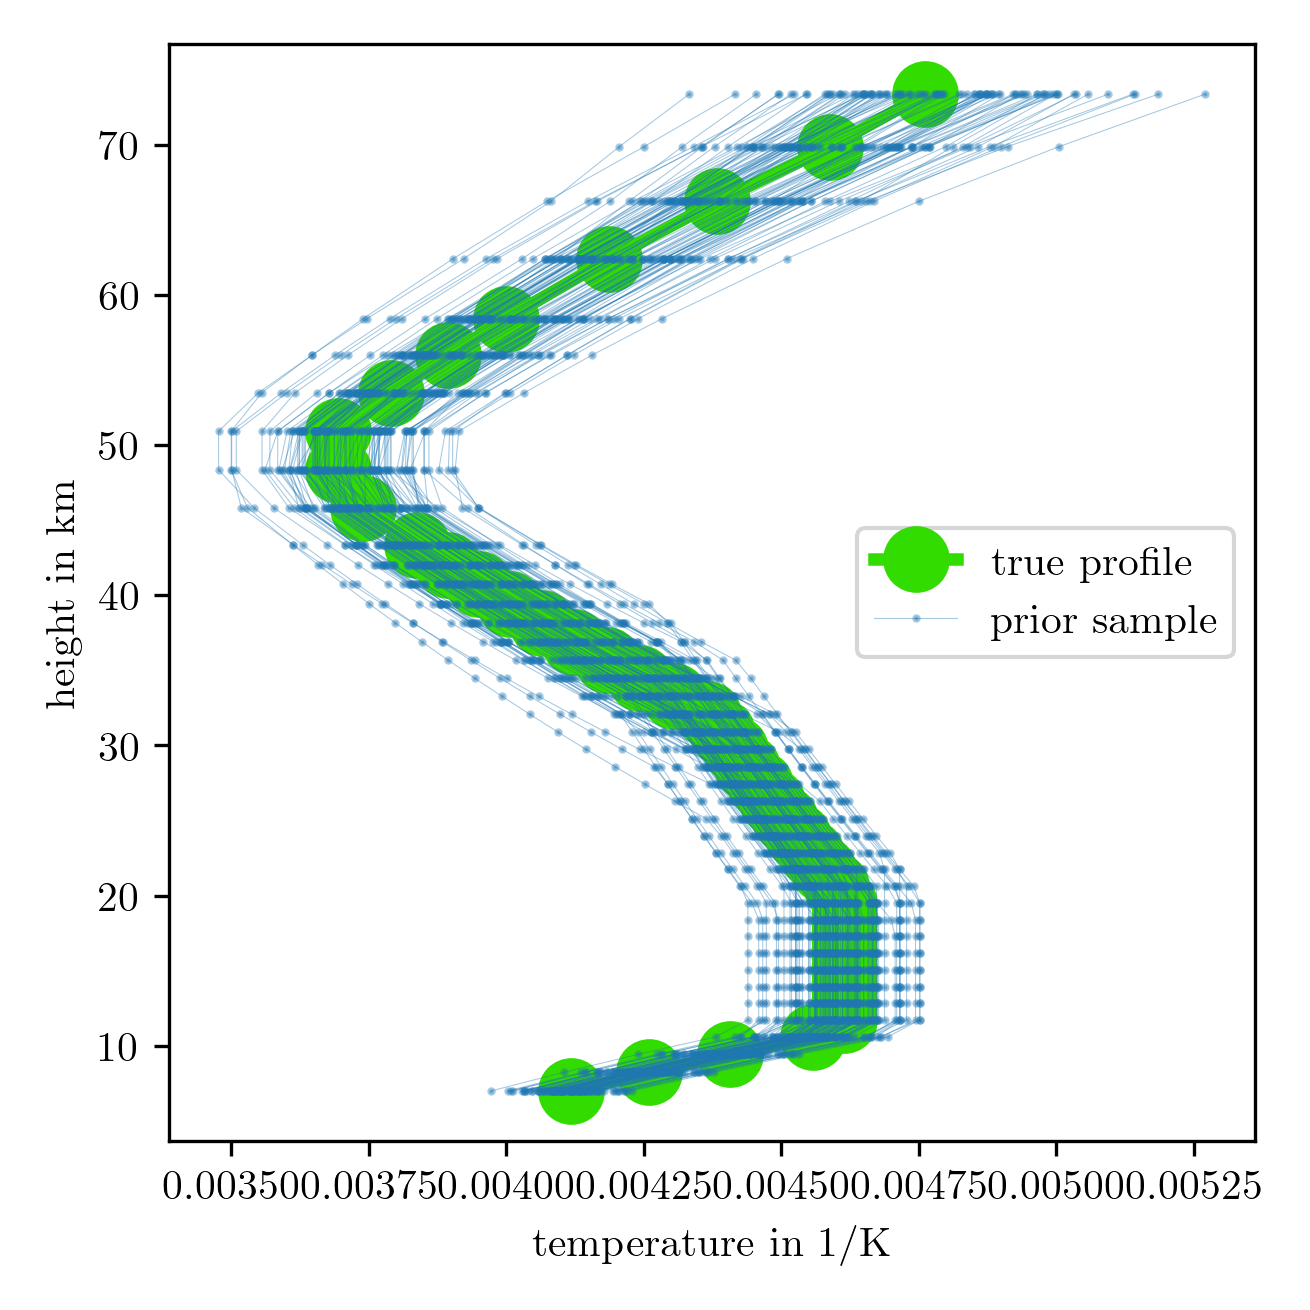
\includegraphics{PriorOverTempPost.png}
	\caption[Prior samples of $1/\bm{T}$]{Prior samples of the inverted temperature profile.}
	\label{fig:OverTempPrior}
\end{figure}

\begin{figure}[ht!]
	\centering
	\includegraphics{TraceTwalk.png}
	\caption[T-walk trace]{Output trace of the t-walk on the posterior distribution $\pi(p_0,b,\bm{h_T},\bm{a}| \gamma,\bm{y})$.}
	\label{fig:TraceTwalk}
\end{figure}



\chapter{Correlation Structure}
\label{ap:Correlation}
In the book Gaussian Markov Random Fields~\cite{rue2005gaussian}, Rue and Held demonstrate that a strong correlation between the hyper-parameter $\mu$ and the latent field $\bm{x}$ can significantly slow down convergence when using samplers, in particularly Gibbs samplers. 
They consider the hierarchical model

\begin{subequations}
\begin{align}
\mu &\sim \mathcal{N}(0, 1) \\
\bm{x} | \mu &\sim \mathcal{N}(\mu \bm{1}, \bm{Q}^{-1}),
\end{align}
\label{eq:rueMod}
\end{subequations}

and apply a Gibbs sampler based on the full conditional distributions
\begin{align}
	\mu^{(k)} | \bm{x}^{(k)} &\sim \mathcal{N} \left( \frac{\bm{1}^T \bm{Q} \bm{x}^{(k-1)}}{1 + \bm{1}^T \bm{Q} \bm{1}}, \, \left(1 + \bm{1}^T \bm{Q} \bm{1} \right)^{-1} \right) \\
	\bm{x}^{(k)} | \mu^{(k)} &\sim \mathcal{N}(\mu^{(k)} \bm{1}, \bm{Q}^{-1}).
\end{align}
As illustrated in Figure~\ref{fig:RueHeld}, when the sampler is restricted to steps only in the $\mu$-direction (horizontal axis) or the $\bm{x}$-direction (vertical axis), it requires many iterations to adequately explore the parameter space. 
This inefficiency arises from the high correlation between $\mu$ and $\bm{x}$, visible in Figure~\ref{fig:RueHeld} as a 'squeeze' of the distribution.
\begin{figure}[ht!]
	\centering
	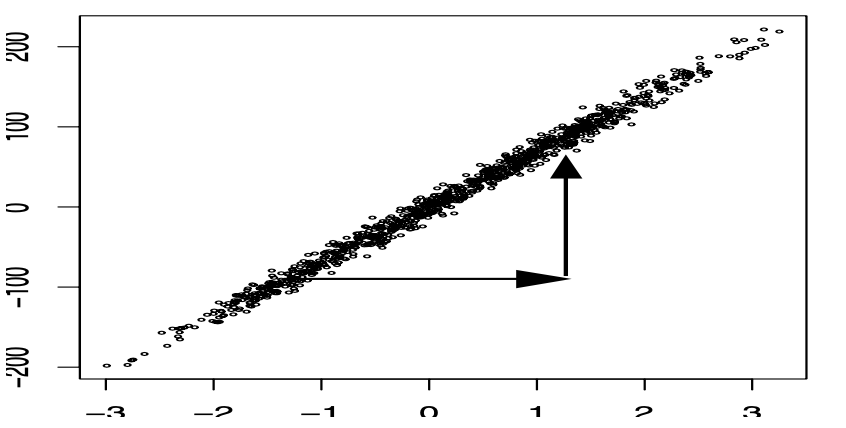
\includegraphics[width = \textwidth]{Figures/RueHeldBookFig.png}
	\caption[Correlation structure in between parameters and hyper-parameters]{The figure taken from~\cite[Figure 4.1 (b)]{rue2005gaussian}, shows samples from a marginal chain for $\mu$ and $\bm{1}^T \bm{Q} \bm{x}^{(k)}$ over 1000 iterations, based on the hierarchical model in Eq.~\ref{eq:rueMod}, with an autoregressive process encoded in $\bm{Q}$. The algorithm updates $\mu$ and $\bm{x}$ successively from their full conditional distributions. The plot displays $(\mu^{(k)}, \bm{1}^T \bm{Q} \bm{x}^{(k)})$, with $\mu^{(k)}$ on the horizontal axis and $\bm{1}^T \bm{Q} \bm{x}^{(k)}$ on the vertical axis. The slow mixing and convergence of $\mu$ result from its strong dependence on $\bm{1}^T \bm{Q} \bm{x}^{(k)}$, while the sampler permits only axis-aligned (horizontal and vertical) and does not allow diagonal moves, as illustrated by the arrows.}
	\label{fig:RueHeld}
\end{figure}

A solution to the slow mixing problem is to update $(\mu, \bm{x})$ jointly.
Since here $\mu$ is one dimensional, effectively only marginal density of $\mu$ is needed.
\begin{align}
	\mu^{\star}  &\sim q (\mu^{\star}|	\mu^{(k-1)} ) \\
	\bm{x}^{(k)} | \mu^{\star} &\sim \mathcal{N} (	\mu^{\star}\bm{1}, \bm{Q}^{-1}) 
\end{align}
With a simple MCMC algorithm targeting  $ \mu$ one can explore the sample space efficiently and only draw a corresponding sample for $\bm{x}$ from its full conditional once, for instance, the proposal $\mu^{\star}$ has been accepted.

\chapter{Mesure theory}
\label{ch:Mesure}
Recall the probability space $(\Omega, \mathcal{F}, \mathbb{P})$, where $\Omega$ denotes the sample space, and $\mathcal{F}$ is a collection of countable subsets $\{ A_n \}_{n \in \mathbb{N}}$ of $\Omega$. Each $A_n \subseteq \Omega$ is called an event, and a map $\mathbb{P} : \mathcal{F} \rightarrow \mathbb{R}$ is referred to as a measure.
In the following, we describe the conditions required for $\mathcal{F}$ to be a $\sigma$-algebra, and for $\mathbb{P}$ to qualify as a probability measure.
We refer to \cite{lawler2016notes} \cite{kopp2004measintprob} for further reading.

\section{probailty measure}
For a probability measure, we require:
\begin{itemize}
	\item $\mathbb{P}(\Omega) = 1$ and $\mathbb{P}(\emptyset) = 0$
	\item $\mathbb{P}(A) \in [0,1]$
	\item $\mathbb{P}(\bigcup_{j \in \mathbb{N}} A_j )= \sum_{j \in \mathbb{N}}  \mathbb{P}(A_j)$ if we have pairwise disjoint sets or $A_i \cap A_j = \emptyset$ for $i \neq j $
\end{itemize}
In other words, the probability assigned to the entire sample space must be equal to one, $\mathbb{P}(\Omega) = 1$, and the probability of the empty set must be zero, $\mathbb{P}(\emptyset) = 0$. For any subset $A \subseteq \Omega$, the probability $\mathbb{P}(A)$ must lie between zero and one, i.e., $\mathbb{P}(A) \in [0,1]$.
If e.g. two subsets $A$ and $B$ are disjoint (i.e., $A \cap B = \emptyset$), then the probability of their union satisfies $\mathbb{P}(A \cup B) = \mathbb{P}(A) + \mathbb{P}(B)$.
This property must also hold for a countable sequence of disjoint sets $\{A_j\}_{j \in \mathbb{N}}$, such that $\mathbb{P}\left( \bigcup_{j \in \mathbb{N}} A_j \right) = \sum_{j \in \mathbb{N}} \mathbb{P}(A_j)$.

\section{$\sigma$-algebra}
A collections of subsets $\mathcal{F}$ is called $\sigma$-algebra if:
\begin{itemize}
	\item $\emptyset, \Omega \in \mathcal{F} $,
	\item if $A \in \mathcal{F} $ then $A^C \coloneqq A / \Omega \in \mathcal{F}$
	\item if $A_1 , A_2, \dots  \in \mathcal{F} $ then $ \bigcup_{j \in \mathbb{N}}  A_j \in  \mathcal{F}$
\end{itemize}
In other words, the empty set $\emptyset$ and the entire sample space $\Omega$ must always be elements of $\mathcal{F}$. If a set $A \in \mathcal{F}$, then its complement $A^C = \Omega \setminus A$ must also be in $\mathcal{F}$. 
If, in terms of a probability measure, we are able to assign a probability $\mathbb{P}(A)$ to an event $A$, we must also be able to assign a probability to the event “not $A$”, i.e., $\mathbb{P}(A^C)$.
Finally, if a countable collection of sets $A_1, A_2, \dots \in \mathcal{F}$, then their union $\bigcup_{j \in \mathbb{N}} A_j$ must also be in $\mathcal{F}$. These three properties define the requirements for $\mathcal{F}$ to be a $\sigma$-algebra.
